\documentclass[12pt, a4paper]{article}

\usepackage[slovak]{babel}
\usepackage[utf8]{inputenc}
\usepackage[T1]{fontenc}
\usepackage{geometry}
\usepackage{graphicx}
\usepackage{hyperref}
\usepackage{csquotes}
\usepackage{listings}
\usepackage{setspace}
\usepackage{xcolor}
\usepackage{enumitem}
\usepackage{multirow}
\usepackage{subcaption}
\usepackage{fancyvrb}
\setstretch{1.25}
\newsavebox\shield
\renewcommand{\lstlistingname}{Kód}

\usepackage[style=iso-numeric,backend=biber]{biblatex}
\addbibresource{references.bib}
\AtBeginBibliography{\small}
\lstset{
	language=bash,
	basicstyle=\ttfamily\footnotesize, 
	extendedchars=true, 
	texcl=true,
	inputencoding=utf8,
	breaklines=true,
	frame=single
}

\geometry{
	a4paper,
	margin=2.5cm,
	top=2.5cm,
	bottom=2.5cm
}

\begin{document}
\begin{titlepage}
    \hspace{0pt}
    \centering
    \vfill
    \large Princípy informačnej bezpečnosti \\
    \vspace{0.4cm}
    \vspace{1cm}
    \large \textbf{Zvýšenie odolnosti webových aplikácií proti útokom typu DDoS, 
          \\za pomoci horizontálneho škálovania  \\}
    \vspace{2.5cm}
    \normalsize Miroslav Hájek \\[0.2cm]
	Akademický rok: 2020 / 2021 \\[0.1cm]
	Fakulta informatiky a informačných technológií, \\
	Slovenská technická univerzita v Bratislave
    \vfill
\end{titlepage}


\pagenumbering{gobble}
\tableofcontents
\newpage
\pagenumbering{arabic}
\setcounter{page}{1}

\section{Dostupnosť ako bezpečnostný atribút}
Zabezpečenie nepretržitého prístupu k webovým službám je očakávanou a takmer nevyhnutnou požiadavkou pre 
akýkoľvek významnejší informačný systém. Predstavuje neoddeliteľnú súčasť obrazu o spoľahlivosti 
ich prevádzkovateľov pôsobiacich vo virtuálnom priestore internetu. Aspekt dostupnosti sa prejavuje tým,
že údaje sú k dispozícii pre autorizovaných používateľov okamžite a bez nečakaných obmedzení   
 \cite{availability}. Odlišná interpretácia definuje pojem dostupnosti ako ochranu proti zlomyseľnému 
zatajovaniu informácií. Spoločným menovateľom pre oba tieto pohľady je dôraz na všadeprítomnosť služby v 
ľubovoľnom čase potreby. Taký stav je vskutku ideálny, ale je možné sa mu aspoň priblížiť predovšetkým 
identifikáciou bodov zlyhania alebo miest prieniku a ich následným systematickým eliminovaním.

Pre bezpečné nakladanie s informáciami nestačí samotná dostupnosť, ale zároveň je potrebné pri návrhu a 
prevádzke systémov myslieť aj na dôvernosť a integritu údajov. Spolu tvoria tradičný model informačnej 
bezpečnosti označovaný ako tzv. \emph{CIA triáda} (Confidentiality, Integrity, Availablity), ktorý sa často 
spolieha na vyváženosť a rovnocennosť týchto troch prvkov \cite{availability}. Nutno poznamenať, 
že to úplne neplatí, pretože nežiadaným znemožnením prístupu k zdrojom sa ich neporušenosť a zabezpečenosť 
proti neoprávnenému prezeraniu, či úprave, stáva bezpredmetná. O dostupnosť sa teda opierajú všetky ďalšie
bezpečnostné predpoklady, ktoré má systém napĺňať.

\subsection{Kľúčový zabezpečovatelia dostupnosti}
Komunikačné technológie často tvoria chrbtovú kosť väčšiny moderných biznisov pričom ich hlavnou úlohou je 
sprostredkovanie informácií naprieč organizáciou a podieľajú sa na riadení podnikových procesov. Okrem 
ľudského kapitálu sa spoliehajú na tri kľúčové prvky: \emph{softvér, hardvér a počítačovú sieť} 
\cite{availability}:

\paragraph{Softvér:}
Softvér je najkritickejším komponentom spomedzi vymenovaných, pretože na základe príkazov v kóde programov 
je ovládaný hardvér a sieťové zariadenia. Všetky potenciálne útoky a ich dopady musia byť riešené primárne 
na úrovni softvéru. Na napadnutie sú využívané zraniteľnosti systému, sprístupnené prelomením nedostatočne 
zabezpečeného verejného rozhrania služieb. Najčastejším cieľom útočníkov je dosiahnutie kontroly nad 
zariadením alebo vyvolaním chaosu vo fungovaní prevádzky. 
 
Zlyhanie programového vybavenia nemusí byť iba v dôsledku nepriaznivých vonkajších vplyvov, ale tiež sa 
prejavujú chyby spôsobené nekorektným návrhom alebo implementáciou systému s odchýlkami od
požadovaného správania. Tieto chyby sú  vnesené neúmyselne najčastejšie programátorom. Počas behu aplikácie 
môžu nastať zlyhania operačného prostredia zapríčinené nedostatkom pamäte pri alokácii, zaplneniu diskového 
úložiska alebo uviaznutím systému. 

\paragraph{Hardvér:}
Poruchy hardvéru bývajú zriedkavejšie, ale o to podstatne fatálnejšie pre celkový chod, keď
výpadok nie je adresovaný redundanciou komponentov. Prinavrátenie do funkčného stavu znamená výmenu
zariadenia za iné prevádzkyschopné, či už dočasnou úpravou fyzickej infraštruktúry alebo neodkladnou 
montážou náhrady. Duplikáciou napr. diskov cez RAID dosiahneme síce vyššiu dostupnosť ale za cenu integrity 
z dôvodu zdvojením dát \cite{availability}, preto je vždy potrebné mať na pamäti vyváženosť bezpečnostných 
vlastností navzájom.

\paragraph{Sieť:}
Obmedzením počítačových sietí je ich priepustnosť podmienená šírkou prenosového pásma a réžiou 
spotrebovanou na obsluhu zvolených komunikačných protokolov. Problémy nastávajú v situáciach, kedy sa 
zahltí sieťová linka. Za normálnych okolností rešpektujú uzly v sieti signalizáciu zaznačenú do 
paketov a prispôsobia rýchlosť vysielania, čím sa po istom čase uľaví náporu. Útočník, ktorý chce saturovať 
serverové pripojenie to  pochopiteľne nerešpektuje a preto by sa nadmerná premávka mala presmerovať a 
filtrovať. Pokiaľ bude smerovač vystavený niekoľkonásobnej záťaži než je schopný podporovať, určite vyvolá 
straty paketov a zvýšenú latenciu.

\subsection{Dôvody viktimizácie prevádzkovateľov}
Nedostupnosť služieb máva za následok, buď priame škody v podobe finančných strát alebo vplýva na 
pošramotenie nadobudnutej reputácie u klientov, ktorí si zlyhanie môžu spájať so stratou spoľahlivosti a 
dôveryhodnosti služby. Poškodenie reputácie sa radí so 47\% medzi najväčšie obavy firiem počas 
kybernetického útoku \cite{radware-ddos}. Ďalšími zreteľmi starostí sú potenciálna strata ziskov s 21\%, 
obmedzená dostupnosť s 12\% a zníženie produktivity počas útoku na 7\%. Čím väčší poskytovateľ a 
používanejšia webová stránka, tým rozsiahlejšie sú potenciálne dopady pri neočakávanom vyradení z prevádzky. 
Zároveň dochádza k adekvátnemu navýšeniu zriadenej odolnosti investovanej do predchádzania a aktívnej 
defenzívy proti útokom. 

Motivácie a dôvody stojace za aktivitami úmyselne narúšajúcimi dostupnosť zvolených obetí v podobe
webových aplikácií sa líšia od prípadu k prípadu, ale sú zhrnuteľné do nasledujúcich okruhov 
\cite{why-attack} \cite{ddos-attacks}:
\begin{itemize}
\itemsep0em 
\item \emph{Kapitálové zisky} - nadobudnutie finančnej odplaty od objednávateľa alebo nekalé snahy o 
potopenie konkurencie v ekonomickej súťaži predstavujú významný hnací faktor pre útočníkov. 
Hlavným zámerom je lepšie peňažné zabezpečenie sa nehľadiac na taktiky vynaložené na tento účel. 
Úspešná realizácia vyžaduje značné technické zručnosti, pretože firmám, ktoré sú hlavných cieľom,
ide o veľa. Zvykne sa dotýkať komerčných webstránok alebo služieb finančných inštitúcií (zaznamenané útoky 
na HSBC, BTC a Ethereum burzy), serverov a sieťových zariadení poskytovateľov webhostingu alebo 
internetového pripojenia (Deutsche Telekom, OVH, Dyn) alebo serverov herných spoločností (Steam, Blizzard, 
EA Sports) \cite{why-attack}

\item \emph{Pomsta} - prevažne frustrovaný jednotlivci snažiaci sa o odplatu za vnímanú 
nespravodlivosť, ktorú podľa nich prevádzkovateľ pácha. Počas operácie Payback z roku 2010 bol odplatou
hackerskej skupiny Anonymous, za blokovanie stránok s torentami a pirátskym softvérom, útok odoprenia 
služieb na organizácie chrániace autorské práva. V decembri zhodili stránky MasterCard, Visa, Paypal a 
iných, ktoré vydržiavali donácie organizácii Wikileaks, pretože publikovala prísne tajné informácie
americkej vlády.

\item \emph{Ideologické a politické presvedčenie} - útočník sa snaží dať hlasno najavo svoj nesúhlas s 
ideovo protichodnými názormi a postojmi znefunkčnením alebo poškodením platformy prostredníctvom ktorej 
oponent pôsobí alebo šíri svoj svetonázor. Takáto forma útokov sa označuje tiež za hacktivizmus, ktorého 
prívrženci hájia slobodu slova a právo na súkromie proti nadmernému sledovaniu. Pre predstavu napádaných 
webstránok boli prominentné útoky roku 2016 cielené na skupiny ako Black Lives Matter, Ku Klux Klan, 
Wikileaks, oboch prezidentských kandidátov v USA, taliansku a írsku vládu alebo európsku komisiu. 
\cite{why-attack}

\item \emph{Demonštrácia schopností} - ide o experimentálne útoky so zámerom hackera vyskúšať si nové 
techniky alebo predviesť svoje kompetencie.
 
\item\emph{Kybernetický terorizmus} - útočník je súčasťou vojenskej alebo teroristickej operácie s cieľom
poškodenia nepriateľovi. Kritická infraštruktúra štátu prestavuje najčastejšie zasahovaný cieľ.
\end{itemize}

\subsubsection{Teória rutinných aktivít}
Výber primeranej obete má taktiež svoj podiel na úspešnosti škodlivého zásahu útočníka do prevádzky,
pretože ten sa výrazne nelíši od konvenčného zločinu. Medzi obvykle spomínané zdôvodnenia páchania 
kriminality zo sociologickej perspektívy patrí kriminologická teória známa pod názvom 
\emph{teória rutinných aktivít}. Vysvetľuje predpoklady, aké musí daný subjekt spĺňať nato, aby bol 
zasiahnutý. Vyslovuje, že zločin sa udeje vtedy, keď motivovaný útočník, so sklonmi na páchanie trestnej 
činnosti, príde do stretu s objektom ponechaného bez prítomnosti schopného strážcu \cite{cohen-felson}.

Pokiaľ sú vytvorené priaznivé okolnosti na prelomenie do systému je veľká šanca, že sa motivovaný útočník 
bude snažiť o zneužitie bezpečnostnej diery. Na druhej stane pri absencii jediného kritéria, sa buď 
znižujú šance na viktimizáciu alebo sa úplne vylúčia. Podľa \emph{teórie racionálneho jednania} koná 
útočník pri zvažovaní realizácie svojho činu racionálne, hoc sa jedná o obmedzenú rozumnosť a síce z uhľa 
pohľadu delikventa ide o cieľavedomé rozhodnutie, kde pozitívny obnos prevažuje nad možnými rizikami 
uskutočnenia.

Vhodnosť zamerania sa na zvolenú infraštruktúru pre potenciálneho páchateľa je zachytiteľné kritériami 
\emph{VIVA} (Value, Inetria, Visibility, Accesibility) \cite{why-attack}. V kontexte útokov odmietnutia 
služby sa pod \emph{hodnotou} rozumie dôležitosť rozbitia cieľa pre útočníka, teda či daný internetový 
portál alebo herný server dosahuje dostatočné zisky, aby ich odstavením bola spôsobená dostatočná škoda. 
\emph{Zotrvačnosťou} sa myslí odpor, ktorý kladie infraštruktúra voči útoku rozličnými bezpečnostnými 
mechanizmami. Medzi priamočiare praktiky patrí udržiavanie aktualizovanému systému so zaplátanými 
zraniteľnosťami alebo obmedzením počtu dopytov z jednej adresy. Služby s veľkou zotrvačnosťou sú schopné 
ustáť väčší nápor v prípade napadnutia. \emph{Viditeľnosť} predstavuje rozsah verejnej prístupnosti a 
známosti webstránky. \emph{Prístupnosť} značí jednoduchosť v dosiahnutí vytýčených sieťových 
uzlov, ktoré majú predstavovať obeť, použitou taktikou útoku bez povšimnutia. Rovnako sa spája so 
schopnosťou nezanechať stopy na mieste činu následkom neprítomnosti mechanizmu monitorovania a detekcie 
narušenia. 

Relatívne vysokou hodnotou, viditeľnosťou a prístupnosťou a nízkou zotrvačnosťou sa cieľ stáva 
exponovanejší a tým žiadanejší pre útočníka. Oproti klasickému zločinu, kedy býva nutná 
prítomnosť páchateľa a obete na jednom mieste, kyberzločin dovoľuje útočníkovi pôsobiť cez internet takmer 
od hocikiaľ a maskovať sa proti odhaleniu.

\subsubsection{Psychologická predeterminácia útočníka}
Pokiaľ by nejestvovali indivíduá so zámerom druhému spôsobiť ujmu vyplývajúcu z nastolených motivačných
faktorov nebolo by ani potrebné sa výrazne zaoberať zvyšovaním odolnosti informačných služieb, či brániť
voči kriminalite ako takej. Určité vzorce ľudského správania naznačujú, že je prakticky nemožné sa pred 
týmito spoločenskými javmi vyhraniť.

Teória diferenciálnej asociácie tvrdí, že v spoločnosti existujú paralelne tak prosociálne, ako aj asociálne 
normy, postoje a spôsoby správania \cite{heretik}, čím sa vysvetľujú trestné činy dostatočne zabezpečených 
jedincov strednej vrstvy. Dochádza u nich k stotožňovaniu sa s antisociálnymi prístupmi na ceste za osobným 
úspechom. Zároveň páchatelia podvedome zľahčujú následky  sociálneho zlyhania v spojitosti s stanovenými 
antikriminálnymi normami. V snahu neutralizovať svoje konanie popierajú zodpovednosti skrývaním sa za 
bezvýchodiskovosť situácie, neuznávajú význam obete  prenášajúc naň vinu a ohraďujú sa konaním v záujme 
vyššieho princípu. Na základe teórie etiketovania je delikvencia len momentálny stav osobnosti, ktorý 
pramálo súvisí s psychickými vlastnosťami a správaním.

Predpokladom na spáchanie kybernetického zločinu sú okrem úvodných pohnútok aj požadované technické 
zručnosti útočníka. Ak pracuje človek radšej sám na seba, a hoc aj nedopatrením má záznam v registri 
trestov, je niekedy motivovaný vlastnou otáznejšou minulosťou voči bežným klientom sa uchýliť k predávaniu 
alebo prenajímaniu kompromitovaných strojov. Hacker si časom vybuduje ilegálny biznis, ktorým si dokáže 
zarobiť uspokojivý obnos \cite{infiltrating-botnet}. Využívané programy sú vymieňané alebo predávané 
sprostredkovane cez fóra, sú reklamované a tamojšími administrátormi overované podobne ako bežný komerčný 
softvér. Na fórach  prebiehajú diskusie a objavujú sa návody k schodným spôsobom ako si dostupný malvér 
sprevádzkovať a upraviť podľa potreby.

Vykonanie útoku so zámerom obmedziť dostupnosť cudzieho systému je podľa platnej legislatívnej úpravy 
na Slovensku trestným činom podľa \emph{§247a Trestného zákona} a obdoby sú zavedené takisto v iných 
právnych poriadkoch (napr. v USA - Computer Fraud and Abuse Act a 18 U.S.C. § 1030, v Nemecku - 
Strafgesetzbuch: §303b  Computersabotage). Činnosť neoprávneného zásahu do počítačového systému spadá v 
podstate do rovnakej oblasti ako poškodenie cudzieho majetku s trestami odňatia slobody pri preukázaní, od 
šiestich mesiacov až po 10 rokov podľa závažnosti \cite{trestny-zakon}. 

\section{Anatómia útokov Denial of Service}
Internet predstavuje prostredie sprístupňujúce na jednej strane ohromnú kvantitu služieb, ale zároveň 
sprostredkúva útočníkom širokú paletu nástrojov umožňujúcich ich odstavenie. Útoky odoprenia služby
- \emph{Denial of Service (DoS)} - spôsobujú nežiaduci zásah do schopnosti legitímneho 
používateľa na prístup k zdrojom dostupných v počítačovej sieti. Zneprístupnenie sa realizuje vyčerpaním 
šírky pásma linky alebo systémových prostriedkov obete, či už CPU, operačnej pamäti alebo priepustnosti 
vstupno-výstupných operácií \cite{ddos-attacks}. Pokiaľ sa na útoku podieľa značný počet zariadení označuje 
sa ako distribuovaný DoS skrátene DDoS. 

Útoky typu DDoS sú na internete obrovským problémom, napriek snahe vyvíjať neustále lepšie 
metódy obrany v reakcii na stále sofistikovanejšie modifikácie techník útokov. V architektúre internetu 
prevládajú prvky so zameraním skôr na efektivitu a spoľahlivosť prenosu paketov medzi koncovými uzlami, než 
na silné zabezpečenie detailnou kontrolou prenášaného toku. Z distribuovanej povahy a autonómie 
administrácie nezávislých samostatných sietí, z ktorých je Internet zložený, a ktoré si riadi 
do veľkej miery každý poskytovateľ pripojenia zvlášť, by bola na systematické celoplošné politiky nevyhnutná 
ťažko dosiahnuteľná širšia dohoda. Zároveň platí, že akokoľvek je cieľový systém ochránený stále závisí od 
úrovne zabezpečenia ostatných uzlov v sieti. Okrem rôznorodého vynútenia pravidiel sú ďalšími predpokladmi 
na degradáciu služieb obmedzené výpočtové zdroje každej entity na trase, hlavne limitované kapacity 
vyrovnávacích pamätí.

Myšlienka uskutočnenia DoS útoku je pomerne priamočiara. Pokiaľ útočník disponuje väčšou celkovou rýchlosťou 
pripojenia, je schopný preťažiť linku obete a tým spomaliť spracovanie oprávnených požiadaviek. Prenesene sa 
uplatňuje zásada, že silnejší pri súboji vyhráva. Strana disponujúca lepším pripojením spravidla predurčí 
stav dostupnosti služby v kritických momentoch. Spustenie útoku iba z jedného akokoľvek výkonného stroja
je pre útočníkov nevýhodné, pretože zmarenie zlovoľnej činnosti spočíva jednoducho vo vyčítaní adresy 
pôvodcu odchytávaním premávky, jeho následne zablokovanie a pridanie na čierne zoznamy. 

\subsection{Botnet}
Centralizované prevedenie útoku odoprenia služby je z dnešného pohľadu nepriechodné. Najčastejšie sa preto 
na znefunkčnenie služby uplatňuje taktika ovládnutia rozsiahlej skupiny zraniteľných počítačov, ktoré dokáže 
útočník ovládať na diaľku a nasadiť do želanej ofenzívy. Napadnuté zariadenia ani ich užívatelia 
častokrát netušia, že sa stali súčasťou takéhoto zoskupenia, ktoré sa označuje ako \emph{botnet}. 
Počítač slúžiaci útočníkovi na naplnenie nekalých úmyslov vzdialeným vykonaných povelov je tzv. \emph{bot}, 
\emph{zombie}, či \emph{dron}. Boti sa správajú ako hybrid viacerých kybernetických hrozieb s pridanou 
hodnotou komunikačného  kanála so schopnosťou koordinácie cez ovládacie miesta. Šíria sa podobne červom, 
skrývajú sa pred detekciou ako vírusy a obsahujú útočne metódy toolkitov \cite{zombie-roundup}. Vlastník 
armády botov je tzv. \emph{botmaster}. Neprávom nadobudnuté výpočtové prostriedky riadi prostredníctvom 
command and control (C\&C) infraštruktúry.

\subsubsection{Komunikácia s botmi}
DDoS útočné siete používajú spravidla tri typy architektúry: \emph{Agent-Handler}, \emph{Internet Relay Chat 
(IRC)} a \emph{webovú architektúru} \cite{ddos-attacks} \cite{botnets}. Model Agent-Handler pozostáva z 
klientov - útočníkov, ktorí sa pripájajú na tzv. handler so zaneseným softvérovým vybavení na zisťovanie 
stavu a koordináciu agentov. Umiestňuje sa spravidla do zariadení s veľkým objemom sieťovej premávky a ich 
strategický výber umožňuje výrazne kamuflovať podozrivú komunikáciu. Terminológia \emph{handler} a 
\emph{agent} sa zvykne zamieňať s \emph{master} a \emph{démon}. 

Medzičlánkom preposielania povelov od botmasterov sa rovnako môže stať verejný IRC server. Vtedy sa jedná o 
architektúru založenú na protokole Internet Relay Chat. Pôvodný účel využitia botov spočíval pri
asistencii moderovania rušných četových miestností IRC kanálov \cite{zombie-roundup}. Jedným z prvých bol 
bot Eggdrop napísaný už v roku 1993. V tom čase začali vznikať boti so zámerom útočiť na ostatných 
používateľov a IRC servery. Dovoľovali útočníkovi ukrytie sa za aktivity bota alebo dokonca za botov na 
viacerých počítačoch, ktorý neboli k útočníkom priamo vystopovateľný. Tým bolo umožnené napádať čím ďalej 
väčšie ciele. 

Agenti sa po pridaní k botnetu ohlásia na dezignovaný IRC kanál a ďalej prijímajú a posielajú správy 
cezeň. Tento spôsob je lákavý pre jednoduchosť komunikácie v podobe krátkych textových správ príkazov a 
dostatočnú anonymitu bez silnej autentifikácie. Útočník nemusí udržiavať zoznam dostupných agentov, keďže po 
prihlásení sa na server vie zobraziť všetkých podriadených botov. Pre zložitejšie odhalenie napomáha 
využitie známych portov pre IRC (6667/TCP), pomerne veľká prevádzka na známych IRC serveroch a technika 
\enquote{preskakovania medzi kanálmi} (channel hoping), kedy botmaster využíva zvolený IRC kanál iba na 
krátke obdobie.

Najpoužívanejším modelom je síce pre svoju flexibilitu IRC forma komunikácie, ale v posledných rokoch sa 
objavujú botnety založené na webových aplikáciach. Boty posielajú webovému serveru pravidelne informácie o 
svojom stave. Ovládané sú cez komplexné PHP skripty a komunikácia s agentami dokáže byť šifrovaná cez TLS a 
skrývať sa za bežnú webovú prevádzku na portoch 80/TCP, 443/TCP a tým odolávať tým bežným sieťovým filtrom. 
Narozdiel od IRC spočíva ich nesporná výhoda v nemožnosti únosu botnetu od svojho pôvodného tvorcu únosom 
četovej miestnosti.

\subsubsection{Šírenie replikáciou škodlivého kódu}
Nehľadiac na výber spôsobu komunikácie agentov so svojim command and control uzlom, musí ich sieť byť 
dostatočne rozsiahla na to, aby spôsobila znateľnejší dopadu na webové služby. Zároveň by mala disponovať 
metódami vlastnej replikácie sa na priľahlé napadnuteľné počítače. Priebeh rozširovania vplyvu botnetu
nad zväčšujúcou sa skupinou hostiteľov sa odohráva v postupných fázach. 

V prvom rade musí dôjsť k objaveniu zraniteľných hostov, potenciálnych budúcich botov. Útočník si
môže vytipovať vhodnú známu obeť a pokúsiť sa o prevzatie kontroly manuálne, systematickým skúšaním
prelomenia známych zraniteľností konkrétneho systému. Automatizované skripty, ktoré sú umiestňované do už 
nakazených počítačov sa nepotrebujú vopred špecificky zacieliť, ale dokážu si poskladať zoznam IP adries, 
ktoré bude postupne navštevovať a preverovať preddefinované nezaplátané bezpečnostné diery. 

Skenovanie môže prebiehať \textbf{náhodne} \cite{ddos-anatomy-2004}, kedy každý kompromitovaný uzol v sieti 
generuje postupnosť ľubovoľných IP adries. Technika je použiteľná iba pri IPv4, pretože pri hustote 
rozloženia obsadených IPv6 adries by bol tento postup výrazne neefektívny. Náhodné skúšanie hostov
vytvára veľký objem podozrivej sieťovej premávky smerovanej akiste medzi vzdialenými sieťami, 
ktoré normálne nekomunikujú, čím sa zvyšuje šanca na odhalenie takejto aktivity. Keďže nedochádza 
pri skenovaní k synchronizácii medzi infikovanými počítačmi rastie množstvo duplicitných dopytov
na rovnaký už preverený koncový uzol s ich zväčšujúcim sa počtom.

Obdržaním zoznamu počítačov (\textbf{hitlist}) s ľahko prelomiteľnou obranou dokáže botnet usmerniť svoje 
šírenie. Známym vyhľadávačom verejných adries IoT zariadení s konektivitou k Internetu a prehľadom
známych bezpečnostných dier je \verb|shodan.io|. Kolíziam sondovania sa zabraňuje prerozdelením celého 
hitlistu na menšie časti, čím sa zabezpečí, že každý agent overí stroje z presne určeného rozsahu. Nevýhoda 
spočíva v nutnom zostavení celého zoznamu predtým než dôjde k samotnému rozširovaniu útočnej siete. Dôležité 
je zvolenie vhodnej veľkosti jeho dielov na preposielanie. Ak je zoznam rozsiahly tvorí sa značná sieťová 
premávka, krátky zoznam zapríčiní malú finálnu populáciu agentov. 

\textbf{Topologické skenovanie} nasleduje prirodzene vznikajúce komunikácie objavujúce v sieti, aby
sa dosiahlo presnejšie splynutie s bežným tokom paketov. Nakazený hostiteľ v podobe webového servera 
pošle do prehliadača klientov škodlivý kód a za správnych okolností sa ten dokáže dostať na iné webové
servere, ktoré klient prezerá. Spoliehaním sa na správanie používateľov sa výrazne znižuje rýchlosť a 
úplnosť ovládnutia vyhovujúcich obetí a útočník nedokáže šírenie počítačového červa regulovať.

Predošlé varianty skenovania je užitočné upraviť na prehľadávanie cieľov \textbf{v lokálnej podsieti}, 
čím sa dajú nakaziť náchylné počítače za firewallom a agent pritom neprezrádza svoju lokáciu využívaním
nadmernej intersieťovej výmeny správ.   

Nachádzanie vektorov prieniku počas prechádzania zoznamom adries je uskutočňované, buď horizontálne,
napríklad preverovaním rovnakého otvoreného portu, či mierenej zraniteľnosti naprieč všetkými cieľmi, alebo
sa koná vertikálne a síce testovaním širokého spektra malvérom pribalených utilít snažiac sa vniknúť
dnu hocako. S vykonávaním vybranej metódy pomalým tempom má útočník príležitosť zostať nebadaný po dlhšiu
dobu a ponúka sa mu čas na preverenie možností získania kontroly nad systémom. Po fázach náboru a 
vykoristení nového bota sa naň prenáša škodlivý kód pochádzajúci z centrálneho úložiska (červ 1i0n) alebo
sa siahne zo zariadenia, ktoré bol pôvodcom nákazy v predošlom kroku, tzv. \enquote{back-chaining} (červy
Morris, Ramen) \cite{ddos-anatomy-2004}. 

\subsection{Klasifikácia typov DDoS útokov}
Útok odoprenia služby závisí od schopnosti čo najväčšej alebo špeciálne zameranej sieťovej 
premávky, aby informačná služba neakceptovala požiadavky legitímnych žiadateľov. Odohráva sa
privlastnenie si celej vyhradenej linky alebo výpočtového výkonu prevádzkovateľa útočníkom. 
Ak je vyústením prevalcovanie serverovej infraštruktúry obete nedokonalosťou zabezpečovacích 
mechanizmov dochádza k zrušeniu dostupnosti s následkami už uvedenými. Aby sme porozumeli metódam 
efektívnej obrany je nevyhnutné zatriediť a kategorizovať objavujúce sa
hrozby, s ktorými sa ciele DDoS útoku vedia stretnúť. V literatúre existujú rozličné taxonómie 
separujúce problematiku z rôznych uhlov pohľadu \cite{ddos-attacks} \cite{botnets} \cite{ddos-anatomy-2004} 
\cite{csirt-ddos}.

Základné rozdelenie DDoS útokov spočíva v identifikácii ich primárneho vektora. Webová aplikácia
býva zneprístupnená, buď vyčerpaním šírky prenosového pásma hrubou silou záplavy paketov, alebo
vyplytvaním systémových prostriedkov sémantickým útokom na komunikačný protokol.

\textbf{Volumetrické útoky} (veľkoobjemové útoky) saturujú kapacitu linky rozmanitou plejádou nálože. 
Spoločným menovateľom je technika flooding (záplava). Populárnou formou útoku je posielanie UDP datagramov 
na náhodné porty s úmyslom zapríčiniť overovanie, či sú porty otvorené a spôsobiť reakciu 
servera signalizačnými správami ICMP Destination port unreachable. So snahou donútiť systém, aby sa venoval 
predovšetkým záškodníckym spávam útočníka, pracuje tiež záplava paketmi ICMP Echo Request (Ping) 
s následnou odpoveďou ICMP Echo Reply. Na VoIP služby je účinným SIP Flood, ktorý zaplaví SIP proxy s
falošnými správami pre začatie hovoru SIP INVITE \cite{botnets}. Webový aplikačný server je možné zahltiť 
záplavou HTTP(S) požiadaviek GET alebo POST na náhodné alebo existujúce URI webstránky. Dopytovanie sa na 
neexistujúcu cestu okamžite vráti stavový kód rádu 400 pre  chybu klienta, ale rovnako sa bude server 
musieť zaoberať spracovaním takejto požiadavky, len sa stáva jednoduchšie pozorovateľnou z prístupových 
logov. 

\textbf{Protokolové útoky} sa priživujú na zraniteľnosti v návrhu komunikačného protokolu na transportnej
až aplikačnej vrstve OSI, ktoré spoliehajú na priebežné ukladanie stavových informácii o naviazaných
reláciach. Rozšírené sú taktiky na zneužitie časovačov stavového automatu protokolu TCP a príznakov v TCP 
segmentoch, ktorými sa odosielateľ a prijímateľ dohadujú na priebehu výmeny správ. 

Počas TCP SYN Flood je doručené také množstvo podnetov na otvorenie spojenia segmentami s príznakom SYN, 
ktoré vyústi v zaplnenie pamäte vyhradenie na uchovávanie aktívnych relácii. Server je povinný pri 
zahajovaní TCP spojenia cez 3-way handshake a obdržaní SYN odoslať SYN+ACK a počkať stanovenú dobu. Timeout 
býva dostatočný na to, aby dokázal útočník ponechať tabuľku relácií zaplnenú iba svojimi podvratnými 
požiadavkami. Schodnou ochranou je zavedenie tzv. TCP Cookie. Systém po prijatí TCP SYN odošle TCP SYN+ACK a 
nevytvorí v pamäti žiadnu reláciu \cite{csirt-ddos}. Po prijatí právoplatnej odpovede TCP ACK sa spätne 
dopočíta TCP sekvencia paketov a až vtedy sa zaháji spojenie. 

TCP RST útok sa zameriava na rušenie nadviazaných spojení medzi serverom a klientmi, kedy však je
nutné poznať zdrojovú IP adresu klienta, pretože útočník háda začiatkom konverzácie náhodne započaté 
sekvenčné čísla. Ak uspeje preberie reláciu a zruší ju. Za bežných okolností je také niečo ťažko 
spáchateľné, lebo TCP spojenia zvyknú mať krátke trvanie a vznikajú ad-hoc.

Nastavením príznaku PSH je serveru nanútené okamžité vyprázdnenie vyrovnávanie pamäte klientovi
a odoslanie potvrdzujúcej správy ACK. Pri enormnej hromade takýchto výziev nebude schopný server
vybavovať ďalšie požiadavky, čím dôjde k zrušeniu dostupnosti webových a podobných služieb poskytovaných
z daného bodu.

Zlomyseľným zásahom do riadenia toku TCP spojenia predchádzajúceho zahlteniam, presnejšie vyžiadaním a 
udržiavaním nulovej veľkosti okna príjemcu, sa vie útočník obsadiť všetky dostupné spojenia v tabuľke
spojení a tým znemožniť nadviazanie komunikácie so serverom ostatným. Určenie veľmi malej nenulovej
veľkosti okna spôsobí rozdrobenie odpovedí na veľmi malé fragmenty. Prevenciou býva zapojenie Nagelovho
algoritmu (RFC 896) do TCP implementácie, ktorého úlohou je zamedziť veľkej réžii pri posielaní 
miniatúrneho payloadu.

Na relačnej vrstve modelu OSI je vďačným protokolom na útoky spotrebujúce značný výpočtový výkon Secure
Sockets Layer (SSL/TLS). Keďže majorita webových aplikácií v súčastnosti používa HTTPS
je dôležité si uvedomiť, že proces šifrovania spolu s réžiou pri výmene kľúčov v SSL handshaku predstavuje 
pre server násobnú náročnosť oproti klientovi. Znovu sa naskýta prostý útok záplavou iniciácií TLS spojenia
alebo opätovné dohodnutie SSL komunikácie (renegotiation), ktorá zvykne zahŕňať zmenu parametrov šifrovania
alebo vyžiadanie certifikátu servera. Riešením je blokovanie takýchto požiadaviek alebo \enquote{SSL 
offloading} do špecializovaného hardvéru \cite{csirt-ddos}.

Spotrebovanie všetkých ponúkaných spojení HTTP protokolu aplikáciou webového servera sú preferované
tzv. \enquote{low and slow} útokmi. Agent sa maskuje akoby za veľmi pomalú rýchlosť pripojenia,
no v skutočnosti zámerne rozdrobuje svoj dopyt na krátke fragmenty a posiela ich s významným oneskorením,
aby držal spojenie otvorené čo najdlhšie. Dôvody existujúcich obmedzení tkvejú v maximálnom počte 
súborových deskriptorov procesu alebo únosnej hladine bežiacich procesov. Zástupcom tejto skupiny
útokov je Slowloris a R-U-Dead-Yet? (RUDY). Z dôvodu malej generovanej premávky, prechádza pomerne ľahko 
bez povšimnutia, pretože nemá dopad na iné atribúty systému.

Rovnako ako botnety slúžia na zitenzívnenie devastačného prúdu paketov, tak môžu nepriamo zapájať 
do útoku aj malvérom nenakazené počítače technikami odrazu a zosilnenia. Útoky s odrazom (RDoS a DRDoS) 
zapríčiňujú poslanie paketov s podvrhnutou zdrojovou adresou cieľa útoku záchytným bodom (pivotom).
V domnienke správnosti pôvodcu správy sa odpoveď doručí v konečnom dôsledku na obeť. Samo o sebe to nemá až 
taký význam, okrem odklonenia nevyhnutného prúdu odpovedí od skutočných spúšťačov požiadaviek na tretie
strany. Nastavením cieľovej IP adresy na broadcastovú adresu lokálnej podsiete (L2 alebo L3 OSI) sa
útok zosilní, pričom zasiahne všetky počítače v spoločnom broadcastovom segmente siete. Tiež je priechodné 
odrazenie útoku od viacerých reflektorov. Na týchto princípoch fungujú útoky Smurf a Fraggle.

Domain Name System (DNS) amplifikačné útoky využívajú podstatu odrazeného útoku, ale obsahujú obohatenie
zaručeného nárastu veľkosti DNS odpovede voči dopytu. Faktor zväčšenia DNS query response sa pohybuje
od 1,1 pri jednom A zázname (example.net), 2,75 v prípade troch AAAA záznamoch (youtube.com) alebo 
dokonca 3,5 (yahoo.com) pri siedmich štvor-áčkových záznamoch. Protokol DNSSEC ponúka
cez otvorené rekurzívne resolvery až 30-násobnú amplifikáciu \cite{csirt-ddos}, 
z dôvodu početnosti vrátených NS záznamov a digitálnych podpisov v DS a RRSIG záznamoch. 
Nástrojom \verb|dig| sme objavili odpoveď s 24-násobným zväčšením a podobne iné domény dosahovali
amplifikácie bežne v rozsahu 13 - 18-krát:
\begin{lstlisting}
dig +dnssec +trace opendns.com
dig +dnssec @b.root-servers.net opendns.com
\end{lstlisting}

Každoročný prehľad v trendoch kybernetických hrozieb publikovaných európskou inštitúciou ENISA
konštatuje, že takmer 80\% všetkých DDoS útokov v treťom kvartáli 2019 boli TCP SYN záplavy 
\cite{enisa-ddos}, stávajúc sa najpopulárnejším typom útoku spolu s DNS odrazenou amplifikáciou. 
V apríli 2019 bol zaznamenaný SYN Flood útok s prietokom až 580 miliónov paketov za sekundu. Vyskytujú
sa hlavne multivektorové útoky, čím je ich zdolanie komplexnejšie. Zároveň dominovali útoky kratšie
ako 10 minút, ktorých bolo 84\% zo zaznamenaných. Celkovo došlo k nárastu v počte nahlásených útokov
o 241\% oproti rovnakému obdobiu predošlého roku. \cite{enisa-ddos}.

\subsection{Ochrana spevnením sieťovej ochrany}
Obranné mechanizmy na úspešné zvládnutie útokov odoprenia služby rozlišujeme primárne podľa
úrovne pripravenosti reakcie na \textbf{proaktívne} a \textbf{reaktívne} stratégie
\cite{ddos-anatomy-2004}.

\textbf{Prevenciou} sa zabezpečuje systém proti prieniku priebežným monitorovaním
a pravidelným sťahovaním a inštaláciou bezpečnostných záplat. Súčasne sa budujú
bezpečnostné politiky organizácie, ktoré rátajú s klasickými vektormi DDoS útokov a premýšľa sa 
nad adekvátnym minimalizovaním dopadu hrozieb s nimi spojenými. Prakticky osvedčenými 
riešeniami sú \enquote{resource accounting}, čiže účtovanie a limitovanie počtu vyhradených spojení 
pre každú IP adresu pristupujúcu k službe pri maximálnej frekvencii odpovedí od servera, alebo sa využíva 
\enquote{resource muliplication}, kedy sú zdroje systému duplikované na viaceré zariadenia a prichádzajúca 
záťaž je vyvažovaná medzi nimi.

\textbf{Reaktívne spôsoby} sa usilujú o zmiernenie útoku počas jeho konania. Pre automatizované
riadenie defenzívy by mali byť obranné prvky schopné detekcie útoku odlíšením od typickej sieťovej 
premávky s ohľadom na odstránenie vlastnej chybovosti pri identifikácii falošných poplachov
a prehliadnutí škodlivých činností. Zisťovanie prítomnosti pokusov na odoprenie služieb
sa sleduje rozpoznávaním podozrivých vzorov podľa analýzy predošlých útokov alebo
pozorovanie anomálií v komunikácií. Strážny komponent je sústredený na preddefinované scenáre alebo
sa natrénuje na bežnej premávke a spustí varovanie po prekročení prahových hodnôt.

\subsubsection{Remotely Triggered Black Hole} 
Nežiadúcu premávku je vhodné zlikvidovať na okraji autonómneho systému vzdialene spustiteľnou čiernou dierou 
(RTBH). Nahlásením zdrojov alebo  častejšie cieľa útoku vie správca siete vložiť do spúšťacieho smerovača 
statickú cestu na virtuálne rozhranie \emph{Null}, ktoré spôsobí zahodenie paketov \cite{RFC5635}. 
Postihnutá služba bude síce odrezaná od Internetu, čiže útočník odoprie dostupnosť pre ostatných 
používateľov, ale zmiernia sa negatívne dopady na zvyšnú infraštruktúru. Na edge routeroch sa musí vopred 
nakonfigurovať statická cesta pre ďalší skok stanovený za black hole a zakázať preň odpovedanie o 
nedosiahnutí cieľa cez ICMP:
\begin{lstlisting}
ip route 192.0.2.1 255.255.255.255 Null0
interface Null0: no ip unreachables
\end{lstlisting}
Na trigger smerovači sa musí aktivovať BGP politika na presmerovanie cesty k obeti 
po obdržaní vloženej statickej cesty so spúšťacou značkou (tagom) a povolenie jej distribúcie
medzi iBGP peerov a zároveň nepropagovanie mimo autonómneho systému \cite{cisco-rtbh}:

\begin{lstlisting}
route-map blackhole
    match tag 66
    set ip next-hop 192.0.2.1
    set origin igp
    set community no-export
router bgp 65535
    redistribute static route-map blackhole
\end{lstlisting}
Poskytovateľ pripojenia môže na podnet zablokovať premávku na obeť známej IP adresy
cez pravidlo na spúšťacom routeri. Uvedená statická cesta musí byť po skončení odobratá zo spúšťacieho 
routera, ktorý rozpošle BGP route withdrawal svojim iBGP peerom:
\begin{lstlisting}
ip route 172.5.23.1 255.255.255.255 Null0 tag 66
\end{lstlisting}

\subsubsection{IP Spoofing}
Na zabránenie spätnej väzby paketov vracajúcej sa naspäť botom útočníka, sa zvykne pri záplavových útokoch 
vložiť do paketu sfalšovaná zdrojová adresa. Vychádza z potreby útočníka zostať v anonymite a prípadne 
zmiasť bezpečnostnú obranu vzbudením dojmu, že nadmerná premávka pochádza od rozptýlených podnecovateľov. 
Spoofing sa hodí u reflektorových útokov alebo v situáciach, kedy si útočník praje, aby bol vinený za 
iniciátora určitý počítač. Prostredníctvom zapojenia Ingress a Egress filtrovania sú poskytovatelia 
pripojenia na trase schopný zabrzdiť škodlivú premávky takmer v zárodku. Ukradnuté zdrojové adresy sa 
pre navodenie dôveryhodnosti vyberajú z rozsahu verejne smerovateľných IP adries (RFC 1918, RFC 3330). 
Privátne adresy sa totiž  štandardne zahadzujú na smerovačoch registrovaním príslušných ACL pravidiel ako 
realizácia \textbf{Egress filtrovania} Uvedená konfigurácia odhodí pakety zo súkromného rozsahu a 
prepustí ostatné \cite{cisco-spoofing-rules}: 
\begin{lstlisting}
access-list 110 deny ip 192.168.0.0 0.0.255.255 any
access-list 110 permit ip any any
\end{lstlisting}

Podvrhnuté IP adresy sa rozlišujú podľa techniky ich selekcie. Najmenej sofistikovaný postup spočíva vo 
vygenerovaní náhodného 32-bitového čísla, ktoré predstavuje spoofovanú zdrojovú adresu. 
Vymyslená IP adresa nesmie byť úplne svojvoľná, ale pochádzať z platných podsieti, pre ktoré router má 
záznam v smerovacej tabuľke alebo sa môže nachádzať niekde po ceste k obeti. \textbf{Ingress filtrovanie}
(RFC 2827) totiž povoľuje v striktnom režime smerovať iba pakety, pre ktoré existuje vo FIB (Forwarding 
information base) tabuľke mapovanie reverznej cesty (Reverse Path Forwarding) cez rovnaké rozhranie. Ak 
nedokáže byť zabezpečené symetrické  smerovanie potom \enquote{loose} mód dovoľuje akceptovať spätnú cestu 
cez ľubovoľné rozhranie smerovača:
\begin{lstlisting}
ip verify unicast reverse-path list           # Strict mode
ip verify unicast source reachable-via any    # Loose mode
\end{lstlisting}
Naproti bežnej predstavy prevláda snaha o zúžitkovanie validných zdrojových adries agentov útočníka,
tam kde je to uskutočniteľné \cite{ddos-anatomy-2004}.

\subsubsection{Linux Netfilter}
Zníženie záťaže na systémové zdroje pridelené na tvorbu paketov odpovede je dosiahnuteľné cez 
\emph{rate limiting}. Linux disponuje v rámci \emph{procfs} (\verb|/proc/sys/net/ipv4/|) premennými 
na obmedzenie rýchlosti pri odpovedaní maskou zvolenými ICMP správami \verb|icmp_ratelimit|, 
\verb|icmp_ratemask| a \verb|icmp_echo_ignore_broadcasts|\footnote{\url{https://
man7.org/linux/man-pages/man7/icmp.7.html}}. Predvolene je frekvencia odpovedí na 
ICMP Destination Unreachable 1 sekunda a ignorujú sa broadcastové správy. Proti SYN záplave sa
systém zabezpečí cez \verb|/etc/sysctl.conf| povolením TCP cookies a limitovaním
počtu otvorených, klientom nepotvrdených TCP spojení \cite{haproxy-ddos}:
\begin{lstlisting}
net.ipv4.tcp_syncookies = 1         # Aktivácia TCP SYN cookie
net.ipv4.tcp_max_syn_backlog = 1024 # Maximálny počet nepotvrdených spojení
net.ipv4.conf.all.rp_filter = 1     # Ingress filter (RPF) proti IP spoofingu  
\end{lstlisting}

Z bezpečnostného hľadiska sa tiež odporúča ponechať pravidlá firewallu na najmenšej úrovni priepustnosti 
smerom dnu. Ak webová aplikácia beží na porte HTTPS/443 a 
administrácia vstupuje na server cez SSH/22 zo stáleho rozsahu adries intranetu, môže jednoduchá 
konfigurácia firewallu vyzerať nasledovne \cite{csirt-hardening}:
\begin{lstlisting}
# Pravidlá pre povolenie prichádzajúcej komunikácie cez SSH, HTTPS
iptables --append INPUT --protocol tcp --dport 443 --jump ACCEPT
iptables --append INPUT --protocol tcp --dport 22 \ 
         --source 192.168.0.0/24 --jump ACCEPT
# Politiky reťazí pravidiel sú zahodiť všetko okrem odchádzajúcich paketov
iptables --policy INPUT DROP
iptables --policy FORWARD DROP
iptables --policy OUTPUT ACCEPT
\end{lstlisting}

\section{Škálovanie webových aplikácií}
Rozvrhnutie architektúry na nasadenie webovej aplikácie, ktorá ustojí legitímnu premávku, ale tiež 
škodlivo nadmerný prúd vykonštruovaných požiadaviek, vyžaduje balans medzi sústredením prostriedkov na 
jednom mieste do homogénneho monolitu a ich parcelovaním znásobením počtu inštancií. Návrhár musí 
nájsť kompromis medzi obstaraním silnejšieho počítača alebo viacerých počítačov. Priklonenie 
sa k vybranej alternatíve predurčí budúce komplikácie pre rozšírenie platformy hosťujúcej webovú 
službu. 

\textbf{Vertikálne škálovanie} spočíva v navyšovaní výpočtovej sily stroja pridaním, urýchlením 
alebo zväčšením kapacity hardvérových komponentov - procesora, pamätí, diskového poľa, či sieťovej karty - 
utesňujúc vzájomnú väzbu dielcov a očakávajúc ich nevyhnutnú vzájomnú kompatibilitu. Uľahčuje sa tým
údržba a kontrola systému, zachovanie konzistentnosti dát bez nutnosti navyše častí na
zabezpečenie ich integrity. Zároveň sa to odráža na nižšej energetickej spotrebe voči 
mnohým spoločne rovnako výkonným duplikátom. Všetko za cenu o poznanie vyšších obstarávacích nákladov tohto 
kompaktného balíka s výhľadom na obmedzený rozsah pre upgrade, vytvárajúc jediný bod zlyhania pre prípadný 
celkový výpadok poskytovanej aplikácie.

\textbf{Horizontálne škálovanie} je oproti vertikálnemu oveľa odolnejšie proti celkovému zlyhaniu služby, 
keďže sa spolieha na viacero paralelne bežiace kópii aplikácie na separátnych zariadeniach. Komponenty sú 
lacnejšie a jednoduchšie na upgrade. Nevyhnutnosťou je spravidla zosieťovanie a distribúcia záťaže úloh 
pomedzi uzly. Zavedením prostredníka takouto reverznou proxy sa zvyšuje réžia pri nadväzovaní spojení 
medzi klientom a serverom. Okrem toho rastie závislosť na externých prepájacích prvkoch a ich zabezpečení.

\subsection{Algoritmy vyvažovania záťaže}
Load balancing spočíva v rovnomernom optimálnom prerozdelení prichádzajúcich úloh 
na spracovanie medzi všetky účastne entity \cite{load-balance-in-distributed-system}. 
Výsledkom je simultánne vykonávanie viacerých požiadaviek, každá vykonávaná pôvodnou rýchlosťou limitovanou
špecifikami každého komponentu osve \cite{haproxy-docs}. Ideálnou symetrizáciou záťaže sa zvyšuje 
priepustnosť a spoľahlivosť, naplno sa využívajú dostupné výpočtové zdroje, zvyšuje sa odolnosť proti chybám 
a rastie stabilita služby. Úspešnosť nasadeného riešenia závisí od zapojenia vhodného algoritmu pre 
konkrétny typ očakávaných pripojení. Najčastejšie sa vyplatí aplikovať dynamické algoritmy so za behu 
upraviteľným váhovaním a riadením od centrálneho uzla - load balancer. Tie berú do úvahy aj momentálne 
informácie o usmerňovanej sieťovej premávke s dostatočne nízkou réžiou, čím dosahujú dobrý pomer medzi 
férovosťou a efektívnosťou.

\paragraph{Round-Robin} prerozdeľuje objavujúce sa požiadavky postupne každému serveru z 
rotujúceho zoznamu započnúc v náhodne zvolenom. Ak sa zariadenia líšia výkonnosťou je vážením dosiahnuteľné
priradenie väčšej záťaže výkonnejším strojom. Napríklad pre priradenie váh trojici serverov $A=4, B=3, C=2$ 
je ich dobrou permutáciou počas plánovacieho cyklu postupnosť $AABABCABC$  \cite{LVS}. Na server pripadne 
množstvo spojení podľa určenej váhy podielom zo sumy všetkých váh: $W_k / \sum_i{W_i}$. Rôznym počtom 
pridelených požiadaviek sa môže prejavovať dynamická nerovnováha medzi servermi, keď je väčšina dopytov s 
rozsiahlou odpoveďou presmerovaná na rovnaký uzol. Časová zložitosť výberu uzla na spracovanie
je $\mathcal{O}(1)$, pretože sa vyberie ďalší v poradí zo zoznamu.

\paragraph{Least Connections} priradí požiadavku serveru s najmenším počtom aktívnych spojení. Medzi
servermi s rovnakou záťažou sa môže aplikovať Round-Robin. Odporúča sa využiť v prípadoch, kedy bývajú
spojenia rozlične dlho otvorené, pretože postupné prideľovanie neberie do úvahy rozdielne trvanie takýchto 
relácií a tým sa môže dôjsť k nahromadeniu klientov na málo hostoch. Pri váženej verzii algoritmu, kde
počet aktívnych spojení uzla je $C_i$ a a váha $W_i$, smeruje príchodzie spojenie na taký server $j$, že platí \cite{LVS}: $$\frac{C_j}{W_j} = \min_{1 \leq i \leq n}{\left\{\frac{C_i}{W_i}\right\}}$$
Least Connections má časovú zložitosť $\mathcal{O}(n)$ od počtu serverov, pretože hľadá minimálnu
dĺžku fronty spracúvaných požiadaviek od každého servera. 

\paragraph{Least Time} je menej častá dynamická stratégia, kedy sa vyberá server podľa najmenšieho počtu 
aktívnych spojení a súčasne na základe najnižšej priemernej latencie vyrátanej z času trvania po prijatie
prvého bajtu alebo kompletnej, či nekompletnej odpovede \cite{nginx-http-balancer}.

\paragraph{Random} vylosuje na spracovanie požiadavky náhodný zo skupiny dostupných serverov, 
čo môže viesť ku krátkodobému navýšeniu zaneprázdnenosti jediného servera, zatiaľčo
ostatné sú nečinné. Priemerne sa však každej destinácii dostane rovnaký podiel klientov 
\cite{load-balance-in-distributed-system}. Stratégia sa oplatí využívať v prípade rozsiahlejších 
serverových fariem, kedy znižuje kladivový efekt na frekventovane pridávané a odoberané servery oproti
odlišným metódam. Účinnou modifikáciou je náhodný výber dvoch serverov, z ktorý sa vyberie ten
s menším počtom aktívnych spojení s Least Connections alebo Least Time. Namiesto priklonenia sa
k absolútne najlepšej možnej voľbe pri nekompletnej plánovacej informácii sa algoritmus
\enquote{Power of Two Choices} vyhýba horšej variante výberom lepšej možnosti z dvoch. S väčším počtom
náhodných výberov konverguje práve k Least Connections \cite{power-two-choices} za cenu výkonnosti 
vyvažovania, pretože sa blíži k vyhľadávaniu globálne najkratšej fronty.

\paragraph{Hashing} sa uplatňuje pri voľbe servera na základe vlastností spojenia alebo hlavičky HTTP 
požiadavky. Konzistentné hašovanie dokáže zaručiť, že pri zmene bežiacich serverov sa minimalizuje a 
zrovnomerňuje počet spojení, ktoré budú zaradené na spracovanie inému serveru. Pri prerozdeľovaní 
zahašovaním zdrojovej IP adresy sa klientovi dostáva odpovede zakaždým od rovnakého uzla pokým je v 
prevádzke, čiže dokáže byť uchovaná perzistencia HTTP relácie s cookies. Tento prístup sa nazýva
best-effort \emph{sticky session} \cite{haproxy-docs}, pretože sa klient akoby \enquote{prilepí} na server
z farmy a pokiaľ je to možné výhradne s ním komunikuje. Na druhej strane sa dá uplatniť hašovanie podľa 
URI cieľa požiadavky alebo iného atribútu s dostatočnou variabilitou. Závisí od ponuky konkrétneho 
nasadeného riešenia.

\subsection{Redundancia nižších vrstiev RM OSI}
Odolnosť sieťovej infraštruktúry proti poruchám a výpadkom aktívnych sieťových prvkov, s vedľajším
rovnako dôležitým efektom navýšenia dátového prietoku komunikačných spojov, sa utužuje vyvažovaním záťaže
na nižších vrstvách modelu RM OSI rôznymi metódami. Agregáciou liniek na spojovej vrstve sa vyberá sieťový 
prepoj zo skupiny, ktorým sa paket pošle. Viaccestným smerovaním na sieťovej vrstve sa rozhoduje medzi 
trasami cez ktoré sériu paketov presmerovať. Virtuálny smerovač (IPVS) na transportnej vrstve určí
aktívy uzol spomedzi klastera pod spoločnou IP adresou.

\paragraph{Agregácia liniek} sa uplatňuje pokiaľ nestačí maximálna prenosová rýchlosť
samotného jedného sieťového rozhrania a je nevýhodné, či dokonca nemožné vymeniť sieťovú kartu.
Vtedy sa oplatí zoskupiť niekoľko fyzických rozhraní do jedného logického linku, spôsob nazývaný
ako \enquote{trunking} alebo \enquote{bonding}. Navyšovanie prenosových rýchlostí
medzi generáciami technológii na fyzickej vrstve môže takto prebiehať lineárne. Ak je vyžadovaný
GigabitEthernet (1 Gbit/s), ale nie je k dispozícii, dokáže Trunked Fast Ethernet
zabezpečiť rýchlosti 200 - 800 Mbit/s, v porovnaní s obyčajným 100 Mbit/s Fast Ethernet. 
Rámce sú striedavo posielané aktívnymi redundantnými linkami vrámci zhluku, čím
sa zabezpečí zvýšená dostupnosť a symetrizácia záťaže na participujúcich portoch.

\emph{Link Aggregation Control Protocol} (LACP), ktorý je súčasťou štandardu IEEE 802.3ad, dovoľuje 
sieťovému zariadeniu vyjednanie automatického združenia liniek výmenou LACP paketov medzi partnermi.
Priebežnými keepalive správami kontroluje LACP priechodnosť spoju pre zamedzenie straty paketov
v nefunkčnej linke a overuje chyby spôsobené nesprávnym fyzickým zapojením vznikajúcim prekrížením 
kabeláže: \enquote{loopback links} alebo \enquote{split-trunk}. Prakticky sa na smerovači nastaví kanál do 
ktorého sú pridané porty\footnote{\url{https://www.cisco.com/c/en/us/td/docs/ios/12_2sb/feature/guide/gigeth.html}}:
\begin{lstlisting}
interface port-channel 1
   ip address 192.168.0.1 255.255.255.0
interface range g2/0/0-1
   no ip address
   channel-group 1 mode active
\end{lstlisting}

\paragraph{Viaccestné smerovanie} pridáva spoľahlivosť v miestach, kde vedú do cieľovej destinácie aspoň
dve trasy. \emph{Equal-cost multi-path routing} (ECMP) je stratégia smerovania, kedy sa striedavo posielajú 
pakety cez viaceré ďalšie skoky s rovnako dobrými metrikami cesty. V praxi je tento prístup málo 
uplatňovaný pre komplikácie viažuce sa k dynamickému výberu spomedzi dostupných smerov na rovnomerné 
rozloženie záťaže \cite{RFC2991}. Rozličné spojenia tiež zvyknú mať rôzne veľkosti MTU (maximum transmission 
unit) a variabilné oneskorenia vedúce k zbytočnému preusporiadaniu paketov správy mimo poradia. Pri použití 
mnohých alternatívnych preskakujúcich ciest môže dochádzať k strate paketov. 

Zmiernenie popísaných negatív výberu pre next-hop, ale vyžaduje udržovanie si 
stavu prebiehajúcich tokov alebo zvýšené výpočtové nároky pre voľbu next-hop. \emph{Modulo-N Hash} 
presmeruje paket na cestu podľa identifikátora toku z hlavičky paketu (najčastejšie zdrojová a cieľová 
adresa) modulo počet dostupných skokov. Ak dôjde k zmene musí sa upraviť $(N-1)/N$ tokov
 \cite{RFC2991}. \emph{Hash-Threshold} rovnomerne mapuje uzly do výstupu hašovacej funkcie a podľa 
porovnania hašu identifikátoru toku s hranicami oblasti je zvolený next-hop. Pri zmenách sa upravuje cesta 
štvrtine až polovici tokov. \emph{Highest Random Weight} počíta hash zakaždým zároveň z hlavičky paketu a
kľúča pre next-hop. Zvolí sa ďalší skok s najvyšším výsledným číslom. Za väčšej časovej náročnosti
sa mení pri pridaní alebo odobratí cesty, smer už len $1/N$ tokov. Cisco router využívajúci na smerovanie
OSPFv2 uplatní ECMP jednoduchým nastavením\footnote{\url{https://www.techrepublic.com/article/how-to-configure-equal-cost-multi-path-in-ospf/}}:
\begin{lstlisting}
router ospf 1
maximum-paths 2
\end{lstlisting}

\paragraph{Virtuálny smerovač} zamedzuje oknám v obsluhe IP adresného priestoru udržiavaním viruálnej 
IP adresy, pre ktorú eviduje redundantné aplikačné servery na zabezpečenie vysokej dostupnosti služby. 
Narozdiel od konceptu základnej dostupnosti, kedy sa vyvinie systém spĺňajúci len nevyhnutné funkčné 
požiadavky, prináša vysoká dostupnosť znásobenie počtu komponentov, aby v prípade údržby, chyby alebo 
zlyhania komponentu mohol zaujať miesto obsluhy úloh náhradný prvok. 

Odstránenie jediného bodu zlyhania nadobúda dve podoby konfiguráciami \emph{Active/Standby} a
\emph{Active/Active} \cite{availability}. Odlišujú sa v móde prevádzky záložného riešenia, 
ktoré je buď nečinnou kópiou (Standby) v \enquote{Cold} alebo \enquote{Hot} režime, preberajúce 
zodpovednosť za spracovanie požiadaviek, iba ak toho hlavný člen nie je schopný, alebo 
sa neplytvá žiadnymi zdrojmi a záloha je operatívna (Active) zároveň s primárnou infraštruktúrou. 
Kontinuálna dostupnosť zachádza ešte ďalej so snahou zamaskovať akékoľvek časové prestoje spojené s 
poruchou, či už zámernou krátkodobou vznikajúcou pri údržbe alebo vážnejšou zapríčinenou útokom.

\emph{Virtual Router Redundancy Protocol} (VRRP) umožňuje súhru viacerých uzlov pôsobiacich ako VRRP 
smerovače tvoriace jeden virtuálny router. Spoločne si volia zariadenie zodpovedné za zdieľanú vysoko 
dostupnú IP adresu. Zariadenie vrámci klastera v roli master má najvyššiu prioritu a v pravidelných 
intervaloch (najčastejšie 1 - 5 sekúnd) vysiela obežníkové správy \emph{VRRP Advertisiment} na multicastovú 
adresu 224.0.0.18 \cite{RFC2338}, na ktorú sú prihlásené cez protokol IGMP všetky uzly v klasteri. Po 
inicializácií je hlavný uzol povinný oznámiť všetkým zariadeniam v LAN cez Gratious ARP správu zmena 
vlastníka IP adresy na svoju MAC adresu. Po výpadku, kedy nebol zachytený Advertisiment približne viac ako 
trojnásobok intervalu, nastupuje backup uzol s najbližšou nižšou prioritou a cez Gratious ARP prehodí IP 
adresu na seba. Keepalived je softvérový balík využívajúci Linux Virtual Server kernel modul umožňujúc 
nastaviť dynamický failover virtuálneho smerovača s VRRP \cite{keepalived-docs}:
\begin{lstlisting}
vrrp_instance malina {       # VRRP inštancia
    state MASTER             # štandardný stav inštancie MASTER / BACKUP
    interface eth0           # sieťové rozhranie
    virtual_router_id 1      # VRRP router id pre inštanciu
    priority 100             # priorita VRRP routera 0 - 255
    advert_int 1             # advertisement interval v sekundách
    virtual_ipaddress { 192.168.0.50 } # VRRP virtuálna IP adresa
}
\end{lstlisting}

\paragraph{DNS load balancing} je staršou technikou prerozdelenia záťaže, pričom obľúbenosť tkvie vo 
výraznej jednoduchosti. Doménové meno služby je asociované s viacerými DNS A záznamami pre IPv4 adresy 
alebo AAAA záznamami pre IPv6 adresy. Následne sa vykonáva statický algoritmus round-robin, ktorý
klientom pri DNS dopyte preusporiada zoznam vrátených serverov a klient si vyberá prevažne prvý z nich. 
Nevýhody sa prejavujú v nedostatočnej flexibilite v porovnaní s rovnomernosťou distribúcie záťaže, aká je 
dosiahnuteľná serverovým load balancerom \cite{server-load-balancing}. 

DNS vyvažovanie záťaže sa vyznačuje značnou nepredvídateľnosťou plánovania smerovania 
sieťovej premávky z distribuovanej podstaty činenia rozhodnutí klientmi. Značným problémom je tiež DNS 
caching, ktorého zámer je obmedzenie vyťažovania autoritatívnych DNS serverov resolvermi. Čas zneplatnenie 
záznamu z cache býva výrazne dlhší ako je potrebné  na okamžité zachytenie výpadku alebo rozširovanie 
kapacity serverovej farmy. DNS nerealizuje health-checks serverov a porucha spôsobí, že značné množstvo 
požiadaviek sa stratí, kým sa DNS záznam stihne všade propagovať.

\noindent\begin{minipage}{.48\textwidth}
\begin{lstlisting}[caption=BIND9: nastavenie DNS zóny .home]
zone "home" {
    type master;
    file "/etc/bind/db.home";
}
\end{lstlisting}
\end{minipage}\hfill
\begin{minipage}{.48\textwidth}
\begin{lstlisting}[caption=Priradenie troch DNS A záznamov pre doménu website.home]
website  IN  A  192.168.0.2
         IN  A  192.168.0.3
         IN  A  192.168.0.4
\end{lstlisting}
\end{minipage}

\subsection{Reverzné proxy HAProxy a NGINX}
Horizontálne škálovanie zabezpečuje spolu s vyvažovaním záťaže reverzný proxy server, ktorý je 
transparentným pre klientov využívajúcich webovú službu. Nasadenie reverznej proxy ponúka množstvo výhod 
týkajúcich sa schopnosti zrýchliť čas obratu prerozdelením požiadaviek, ich komprimovaním (gzip), 
dešifrovaním (TLS) a cachovaním. Dokáže do istej miery ochrániť serverovú farmu pred DDoS útokmi s ACL rate 
limiting. Netreba zabúdať, že proxy tvorí úzke hrdlo pre premávku a predstavuje 
centrálny bod zlyhania, ak nie je duplikované.

Obľúbenými open-source riešeniami pre load balancing na transportnej a aplikačnej vrstve sú softvérové
balíky \verb|haproxy| a \verb|nginx|, ktorých konfiguráciu a výkonnosť porovnáme. \emph{HAProxy} počúva na 
spojenia od klientov na ľubovoľnom počte \verb|frontend|, ktoré sú prepojené na zvolený \verb|backend|, 
kde sú umiestnené definície serverov, ktoré majú byť k dispozícii. Medzi základné sekcie patria tiež 
\verb|global| a \verb|defaults| určujúce správanie HAProxy daemona a nastavenia spoločné pre všetky
frontend a backend sekcie.

\emph{NGINX} konfigurácia pozostáva z dvoch hlavných blokov: \verb|events|, ktorý podmieňuje vlastnosti
bežiaceho NGINX ako celku, a kontext \verb|http| obsahujúci direktívy podmieňujúce
spracovanie HTTP(S) požiadaviek. Rozhranie pre pripájanie klientov tvoria virtuálne servery blokmi
\verb|server|, ktoré okrem poskytovania statického a dynamického webového obsahu cez vnorené kontexty 
\verb|location|, dokážu slúžiť ako proxy pre skupinu serverov zhromaždených v \verb|upstream| bloku.
 
\subsubsection{Vyvažovanie záťaže}
V konfiguračných súboroch oboch softvérových balíkov je najprv nutné nastaviť mód prevádzky na L7, 
respektíve L4 load balancing, pre HAProxy s \verb|mode http|, respektíve \verb|mode tcp|, na NGINX 
umiestnením serverov do kontextu \verb|http {}|, resp. \verb|stream {}|. V prevádzke sa nezaobídeme bez 
schopnosti \emph{logging}, ktorá nám umožní vyhodnocovať stav load balancera v reálnom čase a zároveň 
záznamy pre spätnú analýzu odohraných javov po incidente. 

Zvýšenie bezpečnosti systému s HAProxy daemonom sa dosiahne zmenou koreňového adresáru cez príkaz
\verb|chroot|, ktorý predvolene vytvorí symbolický odkaz z interného \verb|/dev/log| na systémový súbor 
\verb|/var/log/haproxy.log|, kam s \verb|log| direktívou nastavíme preposielanie logov z lokálneho 
zariadenia \verb|local0|. Destináciu pre logy na súborovom systému je zameniteľný za IP adresu alebo  
socket \emph{syslog} servera štandardne na porte UDP/514. Pre NGINX podobne určíme cieľový súbor 
prístupových \verb|access_log| a chybových záznamov \verb|error_log|. Možnosť využitia
\emph{syslog} servera je samozrejmosťou: \verb|access_log syslog:server=192.168.1.1|.

\noindent\begin{minipage}{.48\textwidth}
\begin{lstlisting}[caption=HAProxy mód prevádzky a logging]
global
   log /dev/log local0
   chroot /var/lib/haproxy

defaults
  log global
  option httplog  # tcplog
  mode http       # tcp
\end{lstlisting}
\end{minipage}\hfill
\begin{minipage}{.48\textwidth}
\begin{lstlisting}[caption=NGINX mód prevádzky a logging]
worker_processes auto;
events {
   worker_connections 1024;
}
http {  # stream
  access_log /var/log/access.log;
  error_log /var/log/error.log;
}
\end{lstlisting}
\end{minipage}

Aby proxy server reagoval na žiadosti klientov o otvorenie HTTP spojenia musí počúvať na porte 80 
s direktívami \verb|bind *:80|, resp. \verb|listen 80;|. Následne sú všetky na port prichádzajúce 
požiadavky presmerované na skupinu webových serverov, cez \verb|default_backend|, resp. \verb|proxy_pass|, 
pričom aktivujeme vypĺňanie HTTP hlavičky \emph{Forwarded}, čím bude adresa pôvodného klienta 
sprostredkovaná upstream serverom pre účely loggovania.

\noindent\begin{minipage}{.48\textwidth}
\begin{lstlisting}[caption=HAProxy: preposielanie požiadavok na pool serverov za reverznou proxy]
frontend web
    bind *:80
    option forwardfor
    default_backend website
\end{lstlisting}
\end{minipage}\hfill
\begin{minipage}{.48\textwidth}
\begin{lstlisting}[caption=NGINX: preposielanie požiadavok na pool serverov za reverznou proxy]
server {
   listen 80;
   server_name _;
   location / { 
     proxy_pass http://website;
     proxy_set_header Forwarded 
           $proxy_add_forwarded;
   }
}
\end{lstlisting}
\end{minipage}

Algoritmus rozdelenia záťaže medzi webové servery určíme práve v pomenovanej sekcii \verb|backend|, resp.
\verb|upstream|. Najčastejšie aplikované stratégie ako sú Round Robin, Least Connection a Hešovanie, podľa 
zdroja alebo cieľa, sú podporované na HAProxy aj na NGINX. V HAProxy sa nachádzajú pod voľbami pre príkaz 
\verb|balance| s pomenovaniami: \verb|roundrobin|, \verb|leastconn|, \verb|source|, \verb|uri|.
\cite{haproxy-docs} NGINX predvolenie volí stratégiu Round Robin, ktorá sa dá ekvivalentne zmeniť na: 
\verb|least_conn;| \verb|ip_hash;| alebo na \verb|hash $request_uri| \verb|consistent;| 
\cite{nginx-http-balancer}.

Serverom dokážeme obmedziť maximálny počet aktívnych spojení cez \verb|maxconn n|, kedy zvyšné budú čakať
vo fronte čím sa zníži sa nápor na servery. Príznakom \verb|check| povolíme
aktívne \emph{health checks}, alebo je umožnené dočasne vyradiť server z prevádzky priradením 
stavu \verb|backup| alebo \verb|disabled|. Dokonca časovačom \verb|slow_start| zamedzíme nárazovej záťaži
na uzol dopadajúcej v predurčenom intervale po jeho spustení.  Odlišné váhy pre rôzne výkonné servery 
určíme s prepínačom \verb|weight n| \cite{haproxy-docs}.

\noindent\begin{minipage}{.48\textwidth}
\begin{lstlisting}[caption=HAProxy:  vyvažovanie záťaže najmenej spojení na trojicu HTTP serverov]
backend website
    balance leastconn
    server A 192.168.0.2:80
    server B 192.168.0.3:80
    server C 192.168.0.4:80
\end{lstlisting}
\end{minipage}\hfill
\begin{minipage}{.48\textwidth}
\begin{lstlisting}[caption=NGINX: vyvažovanie záťaže najmenej spojení na trojicu HTTP serverov]
upstream website {
    least_conn;
    proxy_http_version 1.1;
    server 192.168.0.2:80;
    server 192.168.0.3:80;
    server 192.168.0.4:80;
}
\end{lstlisting}
\end{minipage}

\newpage
\subsubsection{Ochrana proti DDoS}
Účinnou obranou proti škodlivo nadmernej sieťovej premávke, nielen voči útokom odoprenia služby, je 
zúčtovanie počtu spojení, rýchlosti súsledných dopytov alebo podobné sledovanie vyhradenia proporcie
dostupných zdrojov alokovaných na IP adresu, ako primárneho identifikátora klienta, aby
sa zamedzilo ich vyčerpanie. Do zaznamenanie užívania prostriedkov sa zapájajú pravidlá na zámerné
riadenia prístupu cez \emph{ACL}. 

Najjednoduchšou technikou obrany proti zneužívateľom držiacim úmyselne  dlho otvorené spojenia s 
nekompletnou správou je časovač, ktorého vypršaním sa spojenie automaticky uzavrie so stavovým kódom 408 - 
\emph{Request Timeout} alebo 504 - \emph{Gateway Timeout}, ale to len vtedy ak nie je nekompletná správa 
vložená do vyrovnávacej pamäte a rovno je odoslaná serveru za proxy.

\noindent\begin{minipage}{.48\textwidth}
\begin{lstlisting}[caption=HAProxy: timeout časovače]
timeout connect 10s
timeout client 30s
timeout server 30s
timeout http-request 5s
option http-buffer-request
\end{lstlisting}
\end{minipage}\hfill
\begin{minipage}{.48\textwidth}
\begin{lstlisting}[caption=NGINX: timeout časovače]
proxy_connect_timeout 10s; 
proxy_read_timeout 30s;
proxy_send_timeout 30s; 
client_body_timeout 5s;
client_header_timeout 5s;
\end{lstlisting}
\end{minipage}

Pokiaľ poznáme IP adresy známych narušovateľov môžeme z nich prístup zakázať, alebo naopak dovolíme
pristupovať iba vyhradenému schválenému prefixu\footnote{\url{https://www.nginx.com/blog/mitigating-ddos-attacks-with-nginx-and-nginx-plus/}}. Riadiť prístup dokážeme taktiež špecificky
pre zastaralú HTTP verziu 1.0, nepovolenú metódu PATCH, DELETE, či HTTP hlavičku, najčastejšie podľa 
\emph{User Agent} s neprípustnou alebo neznámou hodnotou.

\noindent\begin{minipage}{.48\textwidth}
\begin{lstlisting}[caption=Haproxy: ACL pre zdrojové adresy]
http-request deny if { 
  src -f deny_list.lst 
}
tcp-request connection accept if { 
  src 192.168.1.0/24
}
\end{lstlisting}
\end{minipage}\hfill
\begin{minipage}{.48\textwidth}
\begin{lstlisting}[caption=NGINX: ACL pre zdrojové adresy]
location / {   # Deny list IP
  deny 123.123.123.0/28; 
}          
location / {   # Allow list IP
  allow 192.168.1.0/24; deny all; 
}
\end{lstlisting}
\end{minipage}

\begin{lstlisting}[caption=HAProxy: Zablokovanie HTTP požiadavky podľa jej atribútov]
http-request deny if HTTP_1.0                  # HTTP verzia 1.0
acl valid_method method GET POST OPTION HEAD
http-request deny if !valid_method             # Nepovolené HTTP metódy
http-request deny if { req.hdr(user-agent) -i -m sub curl }  # User agent
http-request deny unless { req.hdr(user-agent) -m found }
\end{lstlisting}

Aktívnou metódou je využitie vstavaných počítadiel s asociatívnymi tabuľkami, ktoré priraďujú ku kľúču,
IP adrese, štatistiku počtu alebo frekvencie TCP spojení, resp. HTTP požiadaviek. HAProxy má na tento
účel \enquote{stick tables}, ktoré sú nazvateľné po umiestnenie pod separátnu sekci \verb|backend|. Pri
vytvorení určíme, čo do tabuľky bude ukladať, v našom prípade IPv4 adresy \verb|type ip| a vyhradíme miesto
nad maximálny počet záznamov \verb|size 1m|, tomto prípade 1 milión. O čase po akom sa má odstrániť 
nemodifikovaná položka určuje \verb|expire 10s|, čiže podrží najstarší záznam na 10 sekúnd. Argument za
\verb|store| určuje ako hodnotu ku kľúču uložíme: počet HTTP požiadaviek v posuvnom časovom okne 
\verb|http_req_rate(10s)|, počet spojení pre kľúč v tabuľke \verb|conn_cur|, \verb|conn_rate| 
\cite{haproxy-stick-tables}. Počítadlá sú obnovené automaticky cez \verb|track-src0 src|.

\begin{lstlisting}[caption=HAProxy: obmedzenie počtu otvorených spojení na IP adresu na 10 zároveň]
stick-table type ip size 1m expire 10s store conn_cur
tcp-request connection track-sc0 src
tcp-request connection reject if { src_conn_cur ge 10 }
\end{lstlisting}

\begin{lstlisting}[caption=HAProxy: obmedzenie frekvencie pripojení na používateľa]
stick-table type ip size 1m expire 30s store conn_rate(3s)
tcp-request connection track-sc0 src
tcp-request connection reject if { src_conn_rate ge 10 }
\end{lstlisting}

NGINX používa direktívu \verb|limit_req_zone|, ktorou sa pre zónu zdieľanej pamäte nastavia parametre
limitovania požiadaviek, a príkazom \verb|limit_req| sa určí kontext, kde sa má obmedzovanie HTTP požiadaviek 
algoritmom \emph{leaky bucket} aplikovať \cite{nginx-rate-limiting}. Analogicky s \verb|limit_conn_zone| sa 
vyhradí priestor pre tabuľku pripojení a pre konkrétnu URI cestu limitujeme počet TCP spojení, napríklad na 
10 spojení na IP adresu s \verb|limit_conn zone 10|. Premennou \verb|$binary_remote_addr| určíme, že bude za 
kľúč považovať zdrojové IP adresy v binárnom tvare, čím ušetríme úložisko oproti obyčajnej
\verb|$remote_addr|. Zónou zvolíme miesto vyhradené pre tabuľku, pričom stavové informácie pre približne 16 
tisíc IP adries sa zmestia do megabajtu. Ak obmedzíme príchodzie spojenia na jedno za 100 ms s 
\verb|rate=10r/s| a príde ďalšie v kratšom časovom intervale bude odmietnuté s kódom 503 - 
\emph{Service Unavailable}, čo je nežiaduce v prípade, že sa aplikácia dopytuje nárazovo. 

Atribútom \verb|burst=20| sa vytvorí front s 20 miestami pre spojenia prichádzajúce v rýchlejšom slede ako 
umožňuje obmedzovač \cite{nginx-rate-limiting}. Nastanú situácie, kedy si nemôže dovoliť na odpoveď pre 
legitímnu požiadavku čakať, len preto že bola umiestnená do fronty. Parameter \verb|nodelay| presmeruje 
napríklad 20 simultánnych požiadaviek z IP adresy na server okamžite, ale označí front za zaplnený a uvoľní 
sloty postupne podľa \verb|rate| časovača.

\begin{lstlisting}
limit_req_zone $binary_remote_addr zone=one:10m rate=10r/s;
limit_conn_zone $binary_remote_addr zone=addr:10m;
location / { 
    limit_req zone=one burst=20 nodelay;  # 10 požiadaviek za sekundu
    limit_conn addr 10;                   # 10 aktívnych spojení naraz
}
\end{lstlisting}

\subsubsection{SSL Termination}
Výmena nezašifrovaných HTTP správ sa na webe stáva ojedinelejšia, pretože zvýšené bezpečnostné
nároky komunikácie a vynucovanie zabezpečeného TLS/SSL spojenia zo strany webových 
prehliadačov\footnote{\url{https://security.googleblog.com/2018/02/a-secure-web-is-here-to-stay.html}} 
spôsobili rapídny rozmach HTTPS protokolu v posledných rokoch. Dešifrovanie na strane servera prináša však 
so sebou zvýšenú záťaž na spracovanie požiadavky, preto reverzné proxy umožňujú popri symetrizácii záťaže
SSL premávku dešifrovať pred dosiahnutím webového servera a zašifrovať spätnú odpoveď klientovi - 
\emph{TLS Offloading}\footnote{
\url{https://www.haproxy.com/documentation/aloha/12-5/deployment-guides/tls-infrastructure/}}, 
čím je SSL spojenie ukončené už na proxy. Hlavnou výhodou z pohľadu administrácie je 
centralizovaný a konzistentný manažment TLS konfigurácie a súvisiacich mechanizmov. Predovšetkým sa 
zjednodušuje redistribúcia certifikátov, keďže nemusia byť rozšírené na všetky uzly farmy. Okrem ukončenia 
SSL môže load balancer figurovať v režime \emph{TLS Bridging}, čiže správu k serveru opätovne zašifruje
pre medzikontrolu. Z pozície \emph{TLS pass-through} nenaruší šifrovaný kanál, ale k vyvažovaniu záťaže
musí dochádzať na transportnej vrstve.

Certifikát verejného kľúča by sme na produkčnú prevádzku nadobudnúť od certifikačnej autority 
(napr. Let's Encrypt). Na účely testovanie alebo na použitie v uzavretej komunite môžeme vytvoriť
certifikát podpísaný samým sebou - \emph{self-signed certificate} 

\noindent\begin{lstlisting}[caption=OpenSSL požiadavka (CSR) na samo popísanie certifikátu X.509 so súkromným kľúčom RSA o dĺžke 4096 bitov a ročnou platnosťou, basicstyle=\ttfamily\scriptsize]
openssl req -x509 -nodes -newkey rsa:4096 -keyout key.pem -out cert.pem -days 365
\end{lstlisting}

HAProxy\footnote{\url{https://www.haproxy.com/blog/haproxy-ssl-termination/}} 
a NGINX\footnote{\url{https://docs.nginx.com/nginx/admin-guide/security-controls/terminating-ssl-http/}}
umožňujú označiť komunikáciu na otvorenom porte za \verb|ssl| a zahrnúť certifikát a cestu na disku k 
súkromný kľúču určeného na dešifrovanie. U skupiny upstream serverov stačí, aby podporovali 
nezabezpečený HTTP prenos.  
 
\noindent\begin{minipage}{.48\textwidth}
\begin{lstlisting}[caption=HAProxy: TLS termination]
frontend:
    bind *:443 ssl crt website.pem 
backend:
    server A 192.168.1.1:80
\end{lstlisting}
\end{minipage}\hfill
\begin{minipage}{.48\textwidth}
\begin{lstlisting}[caption=NGINX: TLS termination]
server {
    listen 443 ssl;
    ssl_certificate cert.pem;
    ssl_certificate_key key.pem; }
\end{lstlisting}
\end{minipage}

\section{Monitorovanie webovej aplikácie}


\noindent\begin{minipage}{.48\textwidth}
\begin{lstlisting}
frontend stats
    bind *:8404
    stats enable
    stats uri /stats
    stats refresh 10s
\end{lstlisting}
\end{minipage}\hfill
\begin{minipage}{.48\textwidth}
\begin{lstlisting}
location = /basic_status {
    stub_status; 
    allow 127.0.0.1;
    deny all;
}
\end{lstlisting}
\end{minipage}


\begin{lstlisting}
<Location "/server-status">
    SetHandler server-status
    Require ip 127.0.0.1
</Location>
\end{lstlisting}

\subsection{Zabbix}
\begin{figure}[h!]
	\centering
	\begin{subfigure}[t]{.48\textwidth}
  		\centering
  		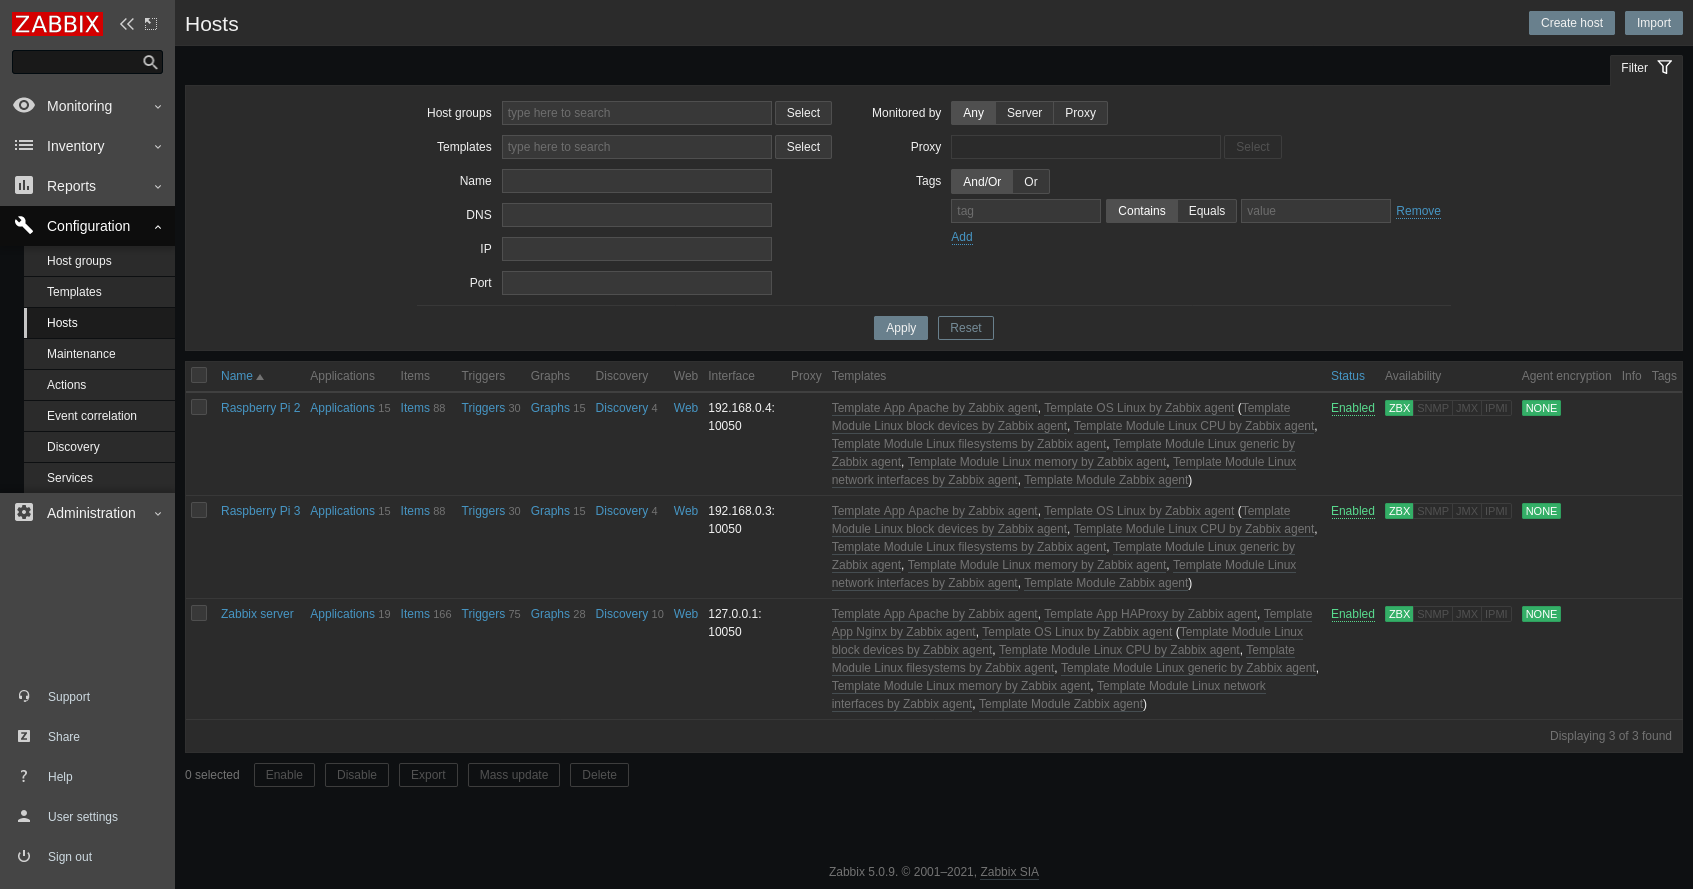
\includegraphics[width=\textwidth]{images/zabbix-host-config.png}
	\end{subfigure}
	\begin{subfigure}[t]{.48\textwidth}
  		\centering
  		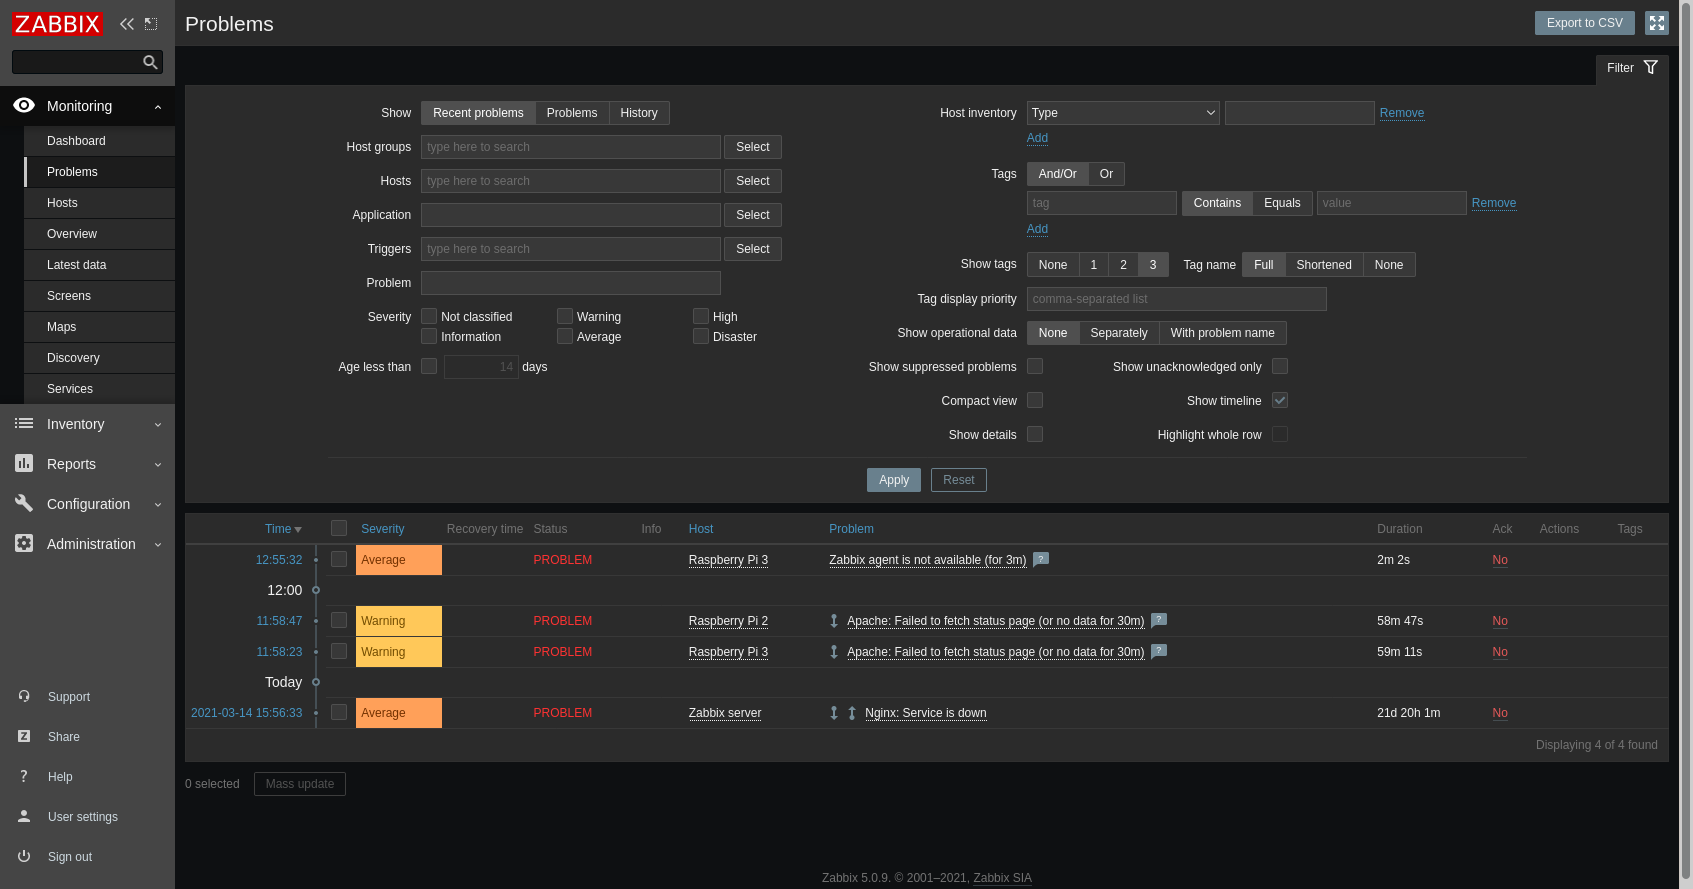
\includegraphics[width=\textwidth]{images/zabbix-problems.png}
	\end{subfigure}
\end{figure}

\begin{figure}[h!]
	\centering
	\begin{subfigure}[t]{.48\textwidth}
  		\centering
  		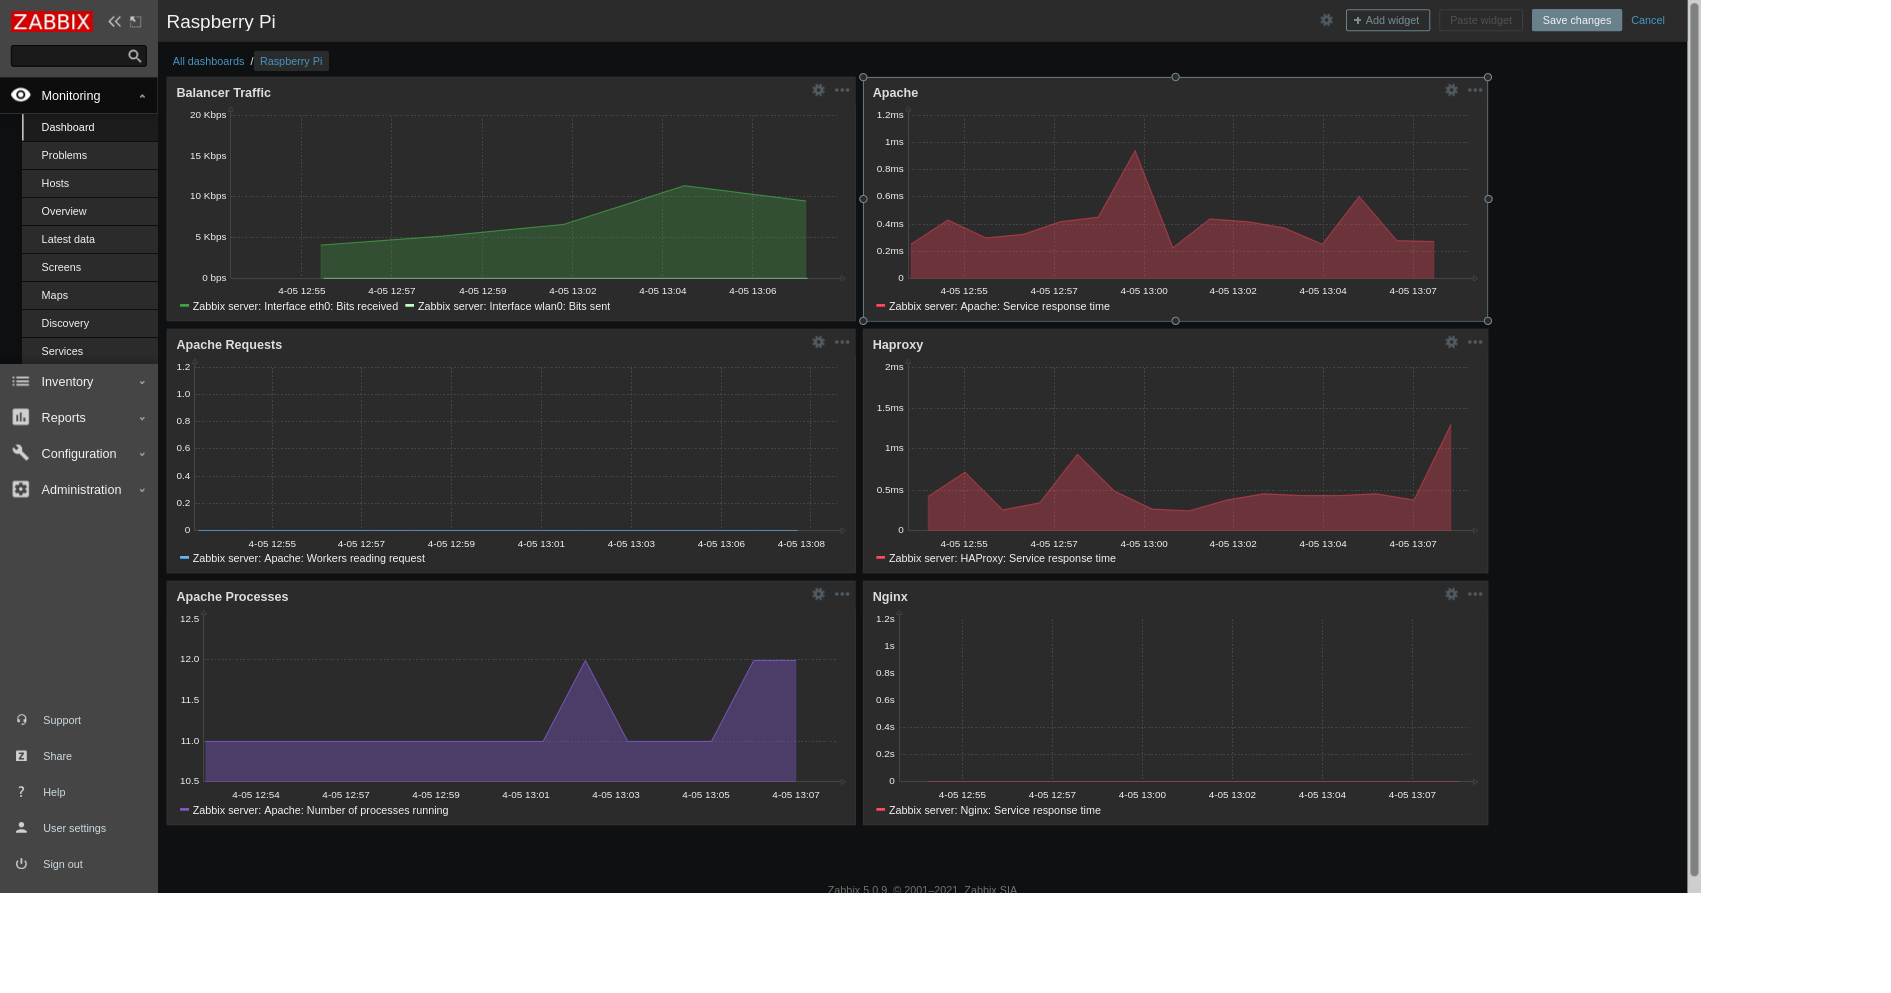
\includegraphics[width=\textwidth]{images/zabbix-dashboard.png}
	\end{subfigure}
	\begin{subfigure}[t]{.48\textwidth}
  		\centering
  		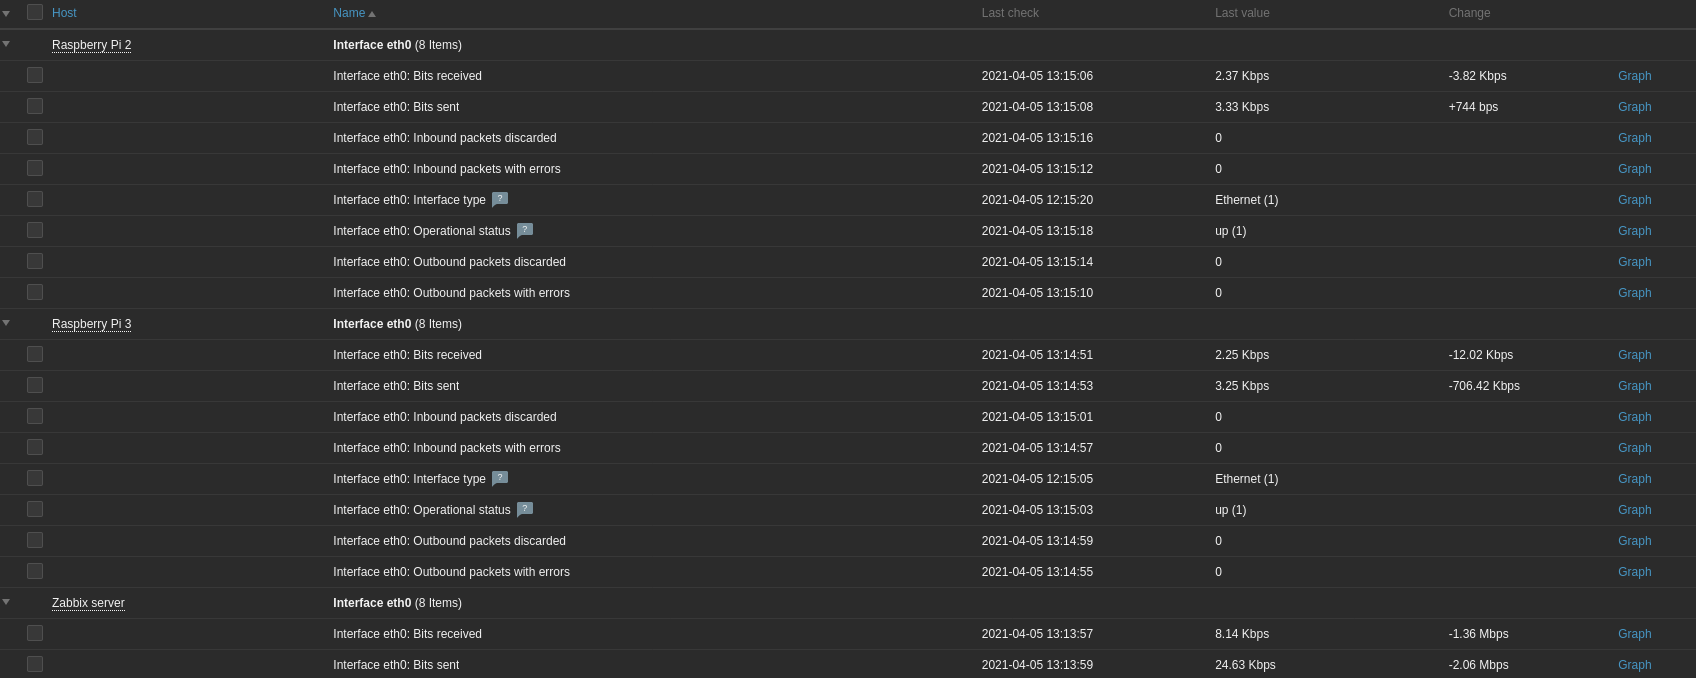
\includegraphics[width=\textwidth]{images/zabbix-eth.png}
	\end{subfigure}
\end{figure}

\begin{figure}[h!]
	\centering
	\begin{subfigure}[t]{\textwidth}
  		\centering
  		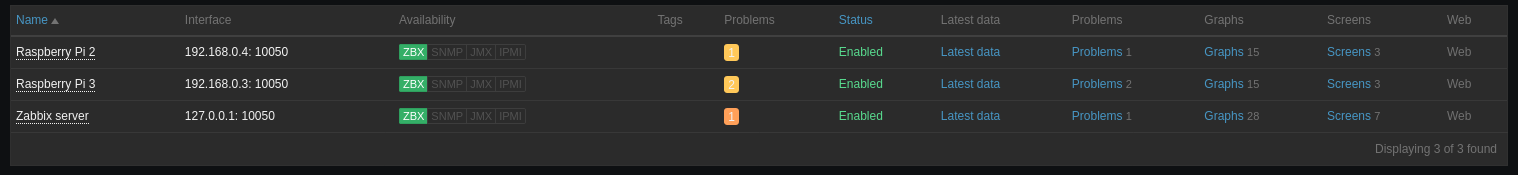
\includegraphics[width=\textwidth]{images/zabbix-hosts.png}
	\end{subfigure}
	\vspace{0.5em}
	\begin{subfigure}[t]{\textwidth}
  		\centering
  		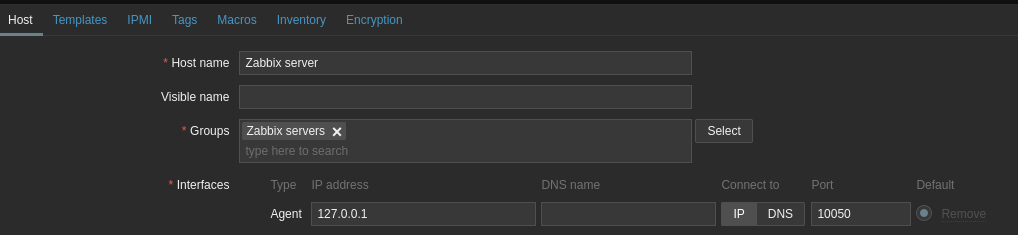
\includegraphics[width=\textwidth]{images/host-config.png}
	\end{subfigure}
	\vspace{0.5em}
	\begin{subfigure}[t]{\textwidth}
  		\centering
  		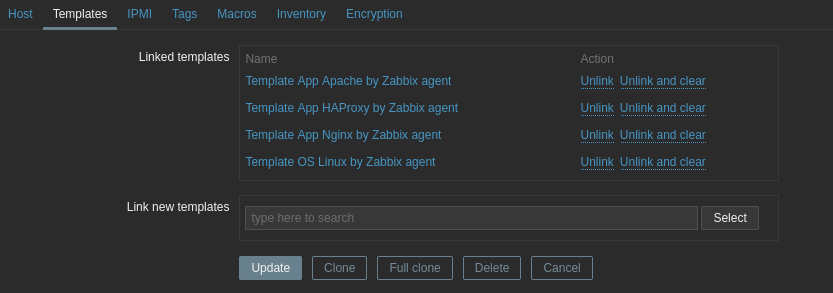
\includegraphics[width=\textwidth]{images/zabbix-templates.png}
	\end{subfigure}
	\vspace{0.5em}
	\begin{subfigure}[t]{\textwidth}
  		\centering
  		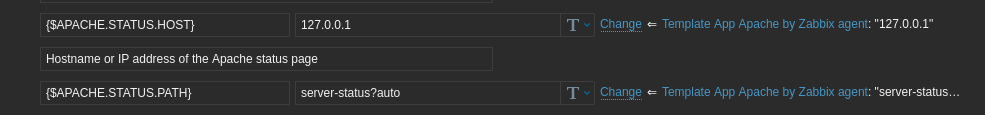
\includegraphics[width=\textwidth]{images/zabbix-macros.png}
	\end{subfigure}
\end{figure}

\subsection{Logging}
\footnote{\url{https://www.haproxy.com/blog/introduction-to-haproxy-logging/}}
\footnote{\url{https://docs.nginx.com/nginx/admin-guide/monitoring/logging/}}
\begin{lstlisting}[caption=Common Log Format]
192.168.0.2 - - [05/Apr/2021 13:45:20 +0200] "GET / HTTP/1.1" 200 1254
\end{lstlisting}

\begin{lstlisting}[caption=Apache Custom Log Format]
website.home:80 192.168.0.2 - - [05/Apr/2021 13:45:20.814 +0200] 
    "GET / HTTP/1.1" 200 351 1254 "-" "Mozilla/5.0"

LogFormat "%v:%p %h %l %u %{%d/%b/%Y %T}t.%{msec_frac}t %{%z}t 
    %D \"%r\" %>s %I %O \"%{Referer}i\" \"%{User-Agent}i\"" custom

<VirtualHost *:80>
   DocumentRoot /var/www/html
   CustomLog ${APACHE_LOG_DIR}/access.log custom
</VirtualHost>
\end{lstlisting}

\begin{lstlisting}[caption=NGINX Custom TCP a HTTP Log]
192.168.0.5 [05/Apr/2021:16:35:30 +0200] TCP 200 465 308 20.960 
192.168.0.5 05/Apr/2021:13:32:15 +0200 "GET / HTTP/1.1" 200 192.168.0.3:80 1294 0.000 0.040 0.040

log_format fmt '$remote_addr $time_local "$request" $status $upstream_addr $upstream_bytes_received $upstream_connect_time $upstream_header_time $upstream_response_time';
log_format fmt '$remote_addr [$time_local] $protocol $status $bytes_sent $bytes_received $session_time';
\end{lstlisting}

\begin{lstlisting}[caption=HAProxy log]
haproxy[2550]: 192.168.0.5:45152 [28/Mar/2021:18:07:58.798] 
    web webservers/A 0/0/5/23/29 200 2862 - - ---- 9/9/8/8/0 0/0 "GET / HTTP/1.1"
\end{lstlisting}



\section{Simulácie útokov a záťažové testy}

\subsection{Sieť na experimenty}
\begin{figure}[h!]
	\centering
	\begin{subfigure}[t]{.48\textwidth}
  		\centering
  		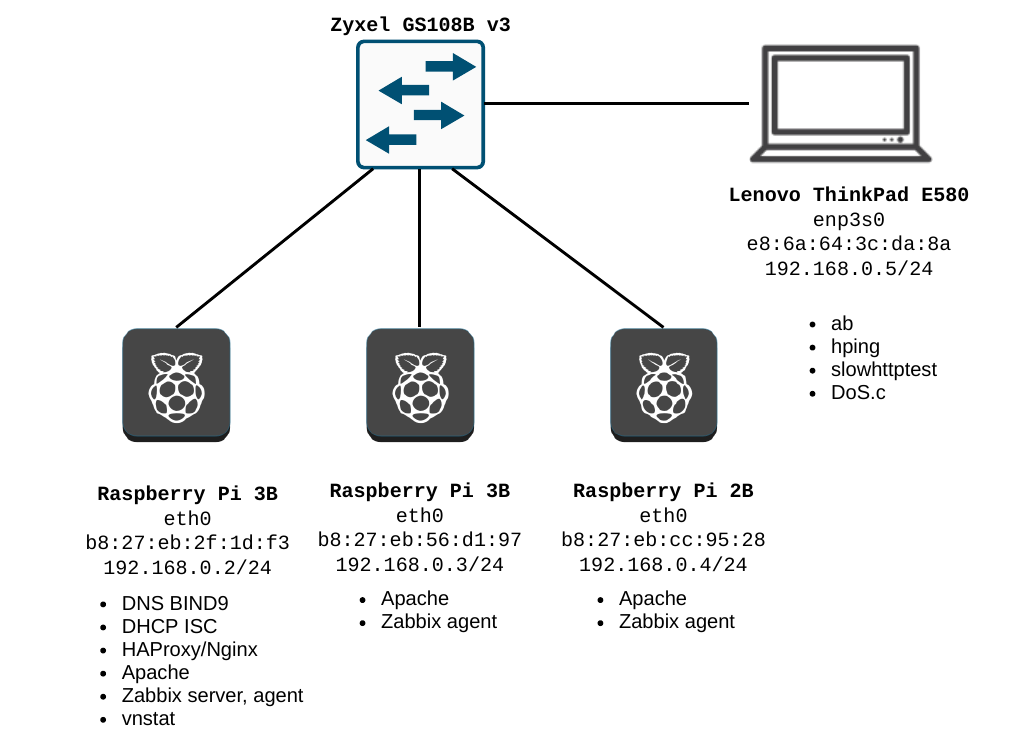
\includegraphics[width=\textwidth]{images/topology.png}
  		\caption{Logická topológia}
	\end{subfigure}
	\begin{subfigure}[t]{.48\textwidth}
  		\centering
  		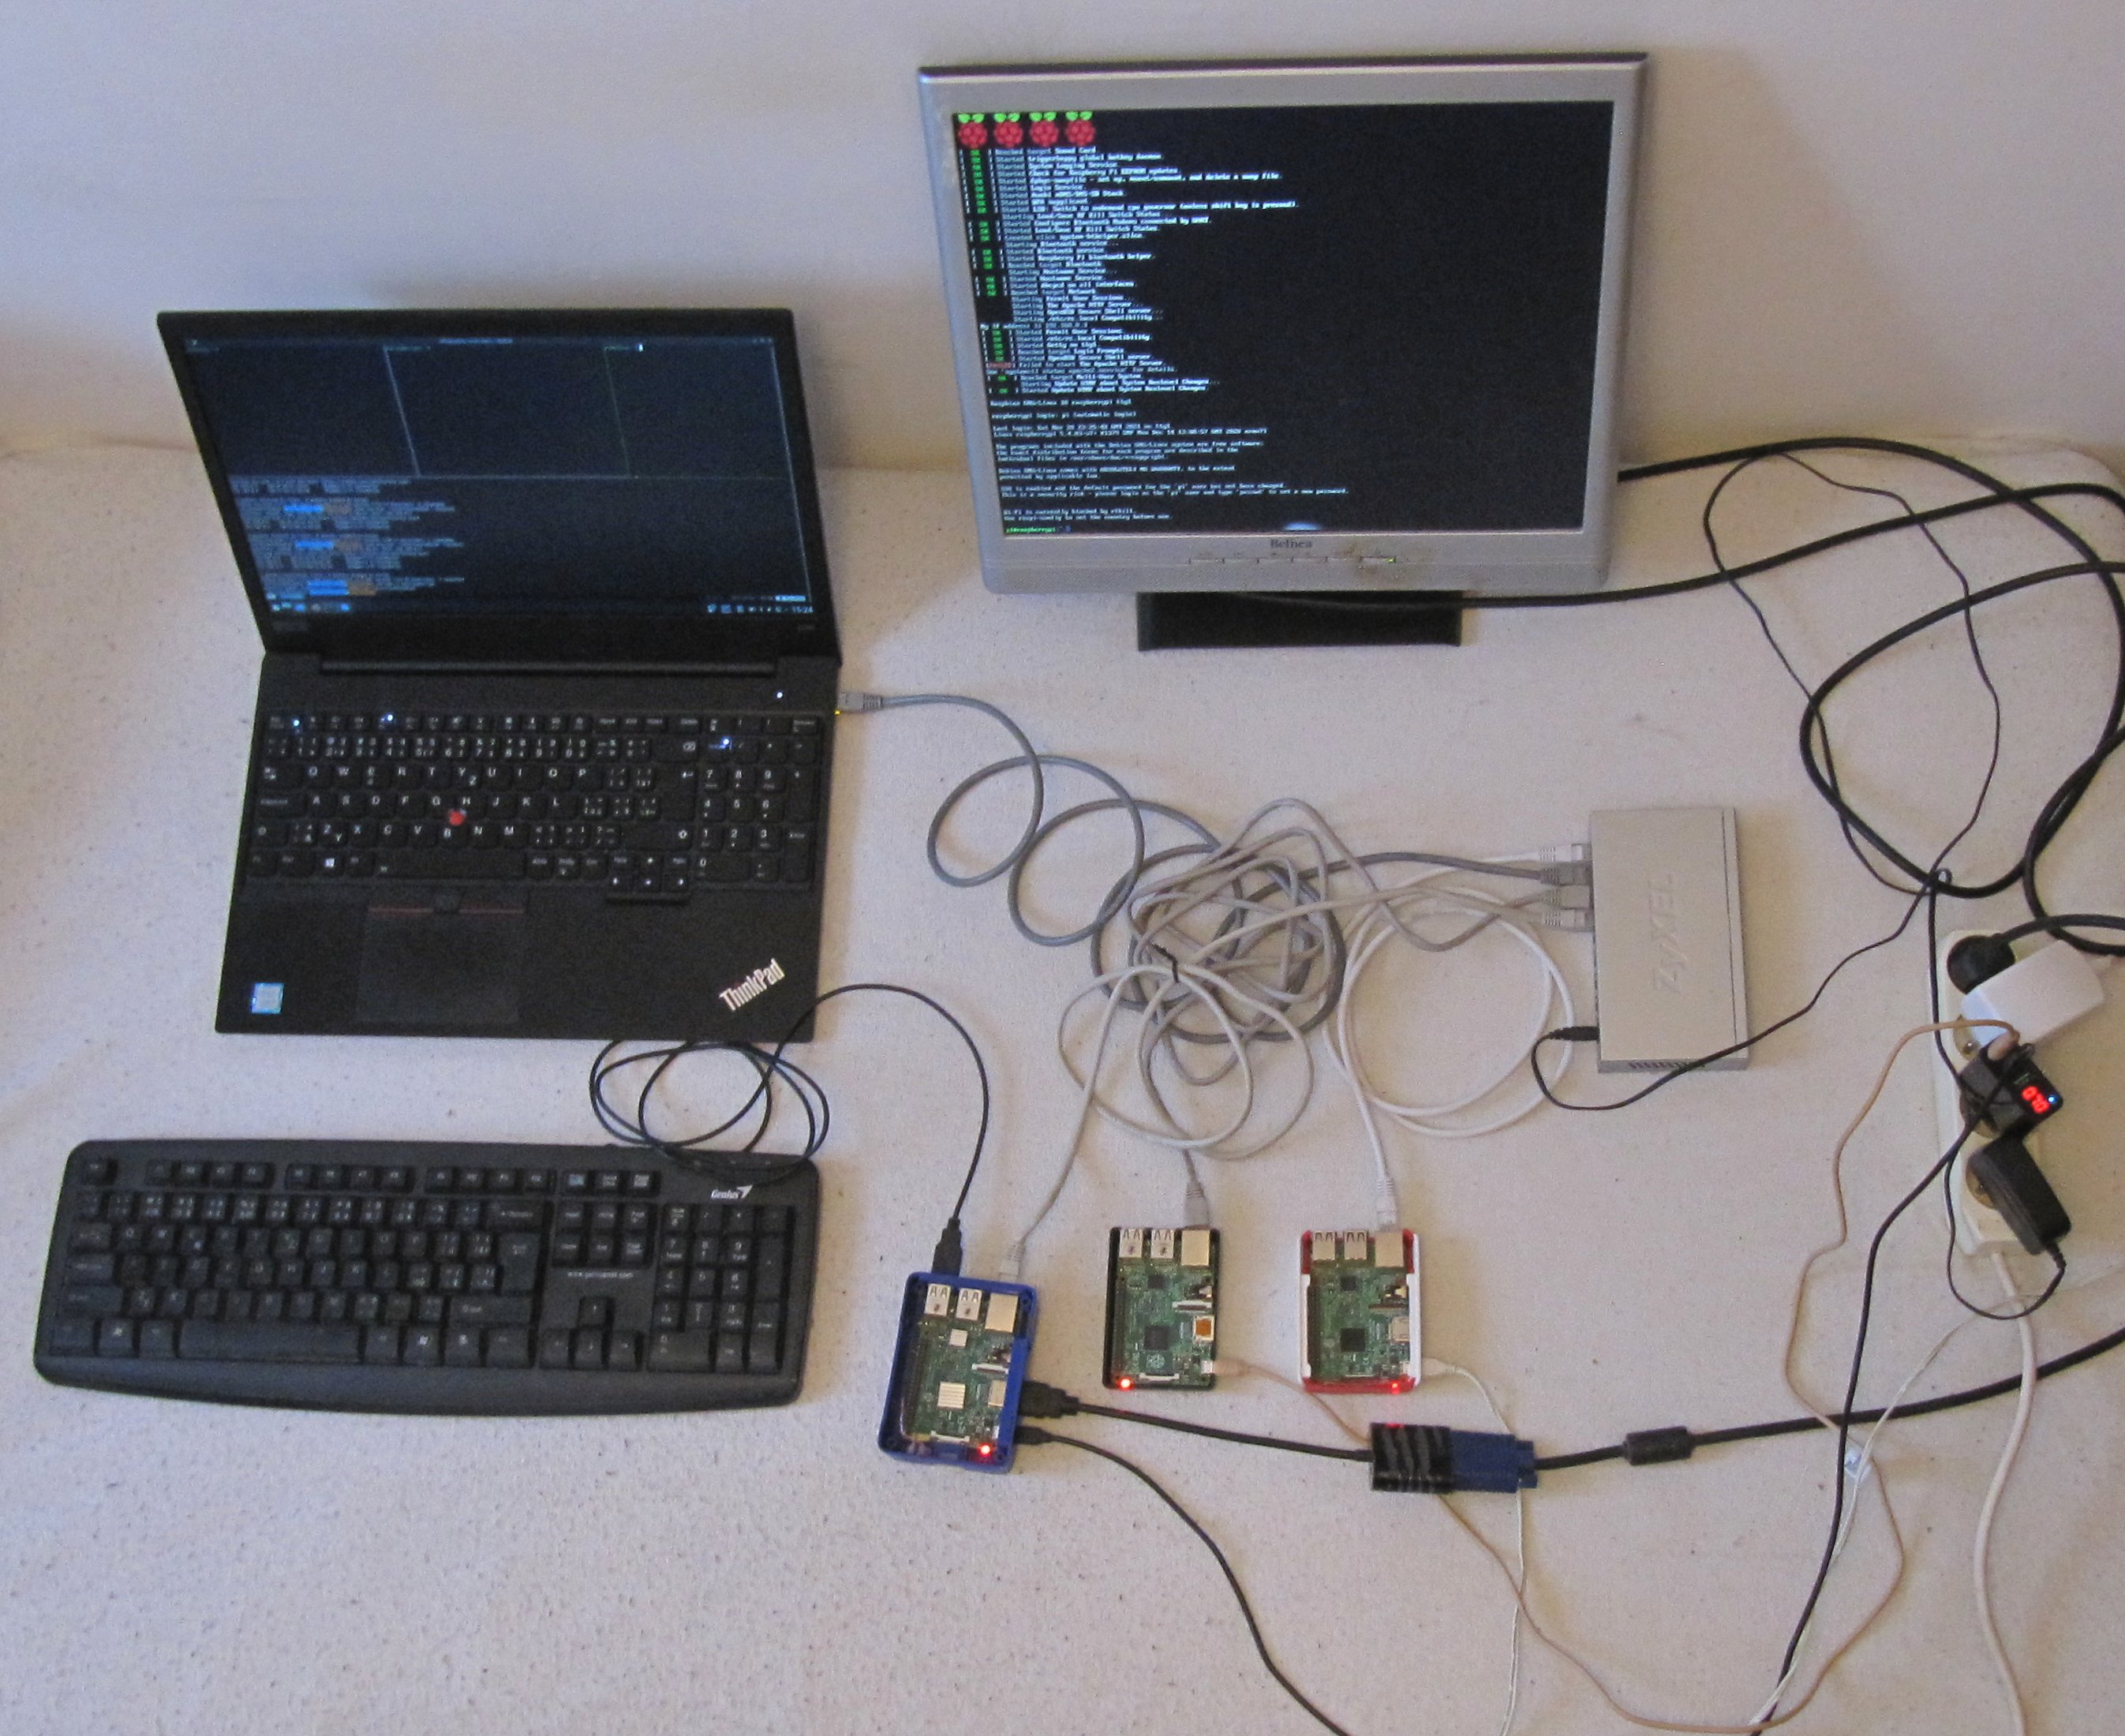
\includegraphics[width=\textwidth]{images/net.JPG}
  		\caption{Fyzická topológia}
	\end{subfigure}
	\caption{Topológia izolovanej siete na experimenty}
\end{figure}

\subsection{HPING na DoS útoky záplavou}
\begin{lstlisting}
hping 192.168.0.2 --udp --flood
hping 192.168.0.2 --icmp --flood  
hping 192.168.0.2 --syn --flood --destport 80
vnstat --traffic
\end{lstlisting}
\begin{table}[h]
\def\arraystretch{1.4}%
\begin{tabular}{|r|r|r|r|r|}
\hline
           & RX {[}Mbit/s{]} & TX {[}Mbit/s{]} & RX {[}pakety/s{]} & TX {[}pakety/s{]} \\ \hline
UDP Flood  & 54,22           & 0,001           & 147345            & 1                 \\ \hline
ICMP Flood & 45,07           & 2,21            & 122483            & 5534              \\ \hline
SYN Flood  & 45,09           & 2,87            & 122539            & 5118              \\ \hline
Slowloris  & 0,14            & 0,13            & 175               & 170               \\ \hline
\end{tabular}
\caption{Dosiahnutá sila útokov s hping odmerané spriemerovaním 5 sekúnd premávky s vnstat na serveri na
sieťovej linke s reálnou šírkou pásma 94.2 Mbit/s}
\end{table}
Na náhodné porty 93 paketov/s, nevráti žiadne pakety pri spoofed ip (nevie cez arp nájsť cieľ)
\begin{figure}[h!]
	\centering
	\begin{subfigure}[t]{.32\textwidth}
  		\centering
  		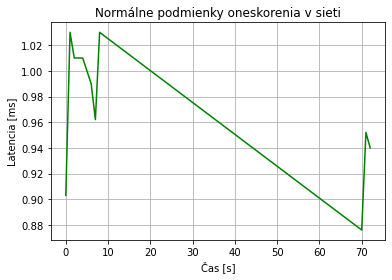
\includegraphics[width=\textwidth]{images/normal-latency.png}
	\end{subfigure}
	\begin{subfigure}[t]{.32\textwidth}
  		\centering
  		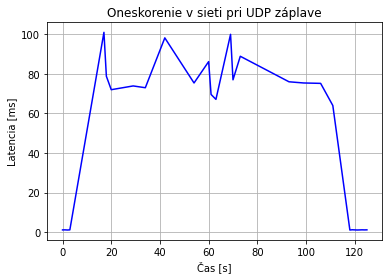
\includegraphics[width=\textwidth]{images/UDP-flood-graph.png}
	\end{subfigure}
	\begin{subfigure}[t]{.32\textwidth}
  		\centering
  		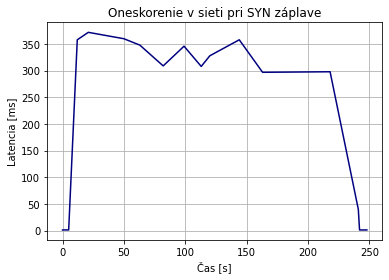
\includegraphics[width=\textwidth]{images/SYN-flood-graph.png}
	\end{subfigure}
\end{figure}

\subsection{Analýza prevedenia DoS útoku záplavou}
\begin{lstlisting}
int s = socket(AF_INET, SOCK_RAW, IPPROTO_RAW);
strcpy(ifr.ifr_name, "enp3s0"); 
ioctl(s, SIOCGIFINDEX, &ifr);
setsockopt(s, SOL_SOCKET, SO_BINDTODEVICE, &ifr);
setsockopt(s, IPPROTO_IP, IP_HDRINCL, (char *)&one, sizeof(one));
\end{lstlisting}
\begin{lstlisting}
in_addr_t ip_random(in_addr_t net, int cidr)
{
    in_addr_t net_mask = (~0 << (32 - cidr));
    in_addr_t host_mask = ~net_mask;
    in_addr_t target_host = 0;
    if (host_mask != 0) target_host = rand() % host_mask;
    return htonl((ntohl(net) & net_mask) | target_host);
}
\end{lstlisting}
\begin{lstlisting}
int s = socket(AF_INET, SOCK_STREAM, 0);
connect(s, (struct sockaddr *)&victim, sizeof(victim))
snprintf(buffer, LEN, "GET /?%d HTTP/1.1\r\n", randint(0, 1000));
send(s, buffer, strlen(buffer), 0);
\end{lstlisting}
\begin{lstlisting}
for (int i = 0; i < CNT; i++) {
    snprintf(buffer, BUF_LEN, "X-a: %d\r\n", randint(1, 50000));
    send(sockets[i], buffer, strlen(buffer), 0);
}
sleep(10);
\end{lstlisting}

\subsection{ApacheBench záťažové testy na load balancer}
\begin{lrbox}{\shield}
\verb|ab -n 1000 -c 100 http://192.168.0.2/|
\end{lrbox}
\begin{figure}[h!]
	\centering
	\begin{subfigure}[t]{.48\textwidth}
  		\centering
  		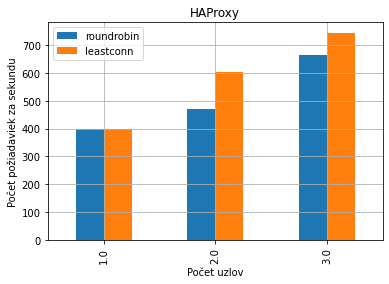
\includegraphics[width=\textwidth]{images/haproxy_ab_1000_100_requests.png}
	\end{subfigure}
	\begin{subfigure}[t]{.48\textwidth}
  		\centering
  		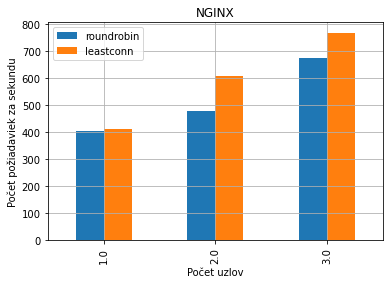
\includegraphics[width=\textwidth]{images/nginx_ab_1000_100_requests.png}
	\end{subfigure}
	\caption{Počet spracovaných požiadaviek za sekundu pre algoritmy vyvažovania 
	záťaže podľa ApacheBench: \usebox{\shield}}
\end{figure}

\begin{figure}[h!]
	\centering
	\begin{subfigure}[t]{.48\textwidth}
  		\centering
  		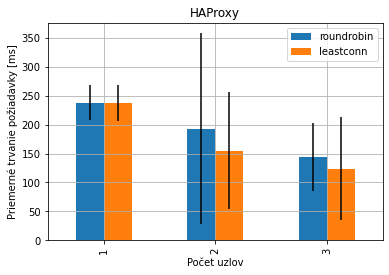
\includegraphics[width=\textwidth]{images/haproxy_ab_1000_100_duration.png}
	\end{subfigure}
	\begin{subfigure}[t]{.48\textwidth}
  		\centering
  		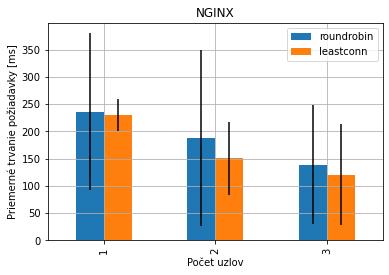
\includegraphics[width=\textwidth]{images/nginx_ab_1000_100_duration.png}
	\end{subfigure}
	\caption{
		Priemerné trvanie požiadaviek pre algoritmy vyvažovania záťaže 
		podľa ApacheBench: \usebox{\shield}}
\end{figure}

\begin{lrbox}{\shield}
\verb|ab -n 10 -c 1 http://192.168.0.2/|
\end{lrbox}
\begin{figure}[h!]
	\centering
	\begin{subfigure}[t]{.25\textwidth}
  		\centering
  		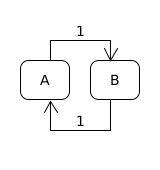
\includegraphics[width=\textwidth]{images/10-uzly-2.png}
	\end{subfigure}
	\begin{subfigure}[t]{.25\textwidth}
  		\centering
  		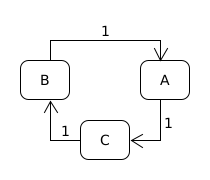
\includegraphics[width=\textwidth]{images/10-uzly-3.png}
	\end{subfigure}
	\caption{Markovove reťazce plánovania pridelenia uzlov na obsluhu požiadaviek
	pri Round Robin aj Least Connections: \usebox{\shield}}
\end{figure}

\begin{lrbox}{\shield}
\verb|ab -n 10000 -c 1000 http://192.168.0.2/|
\end{lrbox}
\begin{figure}[h!]
	\centering
	\begin{subfigure}[t]{.48\textwidth}
  		\centering
  		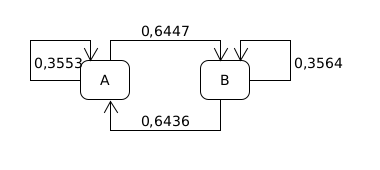
\includegraphics[width=\textwidth]{images/10000-2-RR.png}
  		\caption{Round Robin}
	\end{subfigure}
	\begin{subfigure}[t]{.48\textwidth}
  		\centering
  		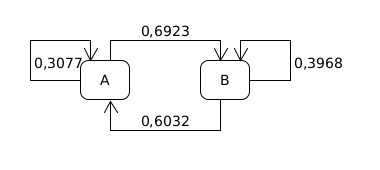
\includegraphics[width=\textwidth]{images/10000-2-LC.png}
  		\caption{Least Connections}
	\end{subfigure}
	\caption{Markovove reťazce plánovania pridelenia uzlov na obsluhu požiadaviek
	pri 2 koncových uzloch: \usebox{\shield}
	}
\end{figure}

\begin{figure}[h!]
	\centering
	\begin{subfigure}[t]{.48\textwidth}
  		\centering
  		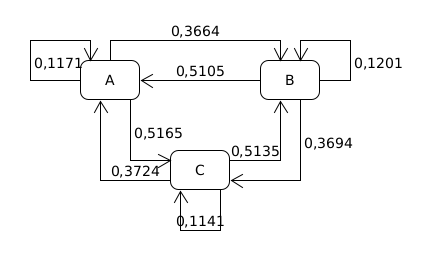
\includegraphics[width=\textwidth]{images/10000-3-RR.png}
  		\caption{Round Robin}
	\end{subfigure}
	\begin{subfigure}[t]{.48\textwidth}
  		\centering
  		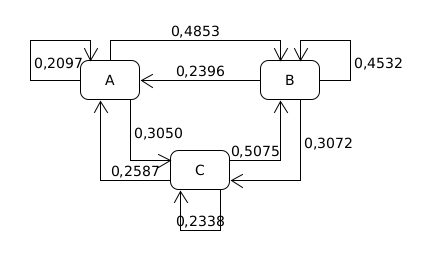
\includegraphics[width=\textwidth]{images/10000-3-LC.png}
  		\caption{Least Connections}
	\end{subfigure}
	\caption{Markovove reťazce plánovania pridelenia uzlov na obsluhu požiadaviek
	pri 3 koncových uzloch: \usebox{\shield}
	}
\end{figure}


\subsection{Slowhttptest Slowloris útok na load balancer}
\begin{lrbox}{\shield}
\verb|slowhttptest -H -c 1000 -i 10 -r 50 -l 180 -g -o stat -u http://192.168.0.2/|
\end{lrbox}
\begin{figure}[h!]
	\centering
	\begin{subfigure}[t]{.48\textwidth}
  		\centering
  		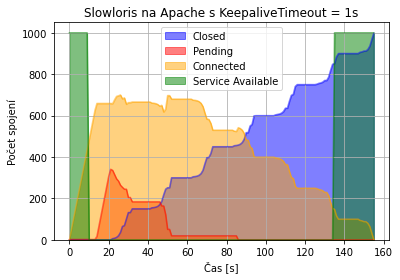
\includegraphics[width=\textwidth]{images/Apache-slowhttptest-1s.png}
	\end{subfigure}
	\begin{subfigure}[t]{.48\textwidth}
  		\centering
  		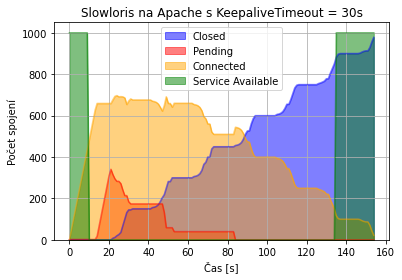
\includegraphics[width=\textwidth]{images/Apache-slowhttptest-30s.png}
	\end{subfigure}
	\caption{Reakcia webového servera Apache na útok SlowLoris pri zmenách Keepalive timeout
	na spojenie: \\ \usebox{\shield}}
\end{figure}
\begin{lstlisting}
  Timeout 300
  KeepAlive On
  MaxKeepAliveRequests 100
  KeepAliveTimeout 5
\end{lstlisting}

\begin{lrbox}{\shield}
\verb|slowhttptest -H -c 10000 -i 10 -r 200 -l 240 -g -o stat -u http://192.168.0.2/|
\end{lrbox}
\begin{figure}[h!]
	\centering
	\begin{subfigure}[t]{.48\textwidth}
  		\centering
  		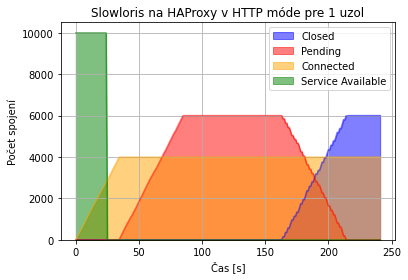
\includegraphics[width=\textwidth]{images/Haproxy-1-http.png}
	\end{subfigure}
	\begin{subfigure}[t]{.48\textwidth}
  		\centering
  		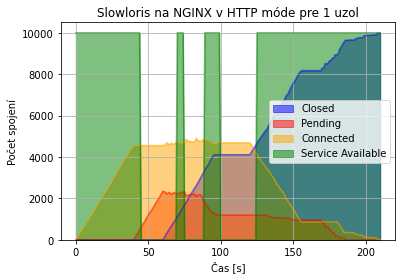
\includegraphics[width=\textwidth]{images/Nginx-1-http.png}
	\end{subfigure}
	\caption{Porovnanie účinkov útoku Slowloris na počet aktívnych spojení a dostupnosť služby
	pri L7 load balancingu na HAProxy a NGINX:\\ 		
	\usebox{\shield}}
\end{figure}

\begin{figure}[h!]
	\centering
	\begin{subfigure}[t]{.32\textwidth}
  		\centering
  		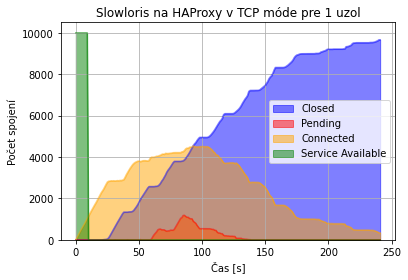
\includegraphics[width=\textwidth]{images/haproxy-1-tcp.png}
	\end{subfigure}
	\begin{subfigure}[t]{.32\textwidth}
  		\centering
  		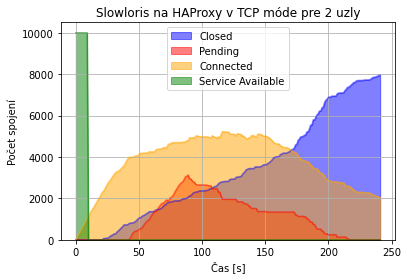
\includegraphics[width=\textwidth]{images/haproxy-2-tcp.png}
	\end{subfigure}
	\begin{subfigure}[t]{.32\textwidth}
  		\centering
  		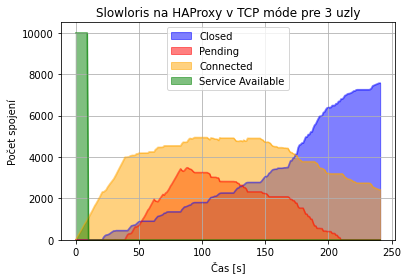
\includegraphics[width=\textwidth]{images/haproxy-3-tcp.png}
	\end{subfigure}
	\begin{subfigure}[t]{.32\textwidth}
  		\centering
  		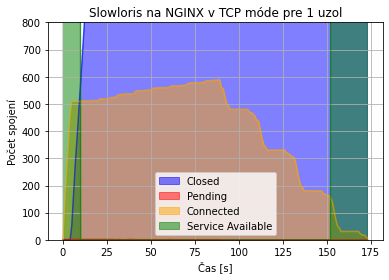
\includegraphics[width=\textwidth]{images/nginx-1-tcp.png}
	\end{subfigure}
	\begin{subfigure}[t]{.32\textwidth}
  		\centering
  		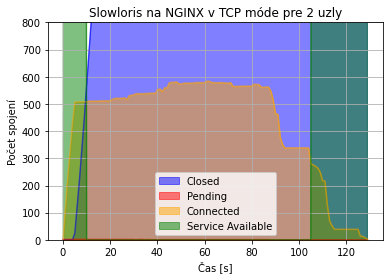
\includegraphics[width=\textwidth]{images/nginx-2-tcp.png}
	\end{subfigure}
	\begin{subfigure}[t]{.32\textwidth}
  		\centering
  		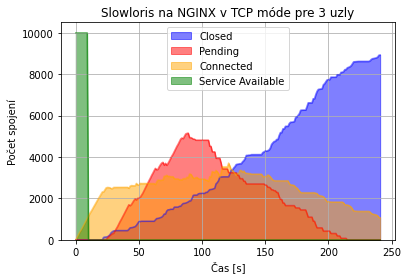
\includegraphics[width=\textwidth]{images/nginx-3-tcp.png}
	\end{subfigure}
\end{figure}

\subsubsection{HTTP hlavičky}
% Zamedzenie zobrazenia http hlavičiek o infraštruktúre (CSIRT-checklist)
\verb|server_tokens off;|
\begin{lstlisting}
<IfModule security2_module>
    SecRuleEngine on
    ServerTokens Min
    SecServerSignature "PIB FIIT STU"
</IfModule>
\end{lstlisting}

\section{Záver}
% Pokrytie témy:
	% analýza možností využitia loadbalancera (haproxy, nginx,...)
	% loadbalancer vs. stateless/statefull spojenia
	% zabezpečenie loadbalancera voči známym typom útokov,
	% zamedzenie inventarizácii architektúry (čo prezradia HTTP hlavičky?)
	% možnosti monitoringu loadbalancera (štatistiky, analýza logov, existencia rozšírení do monitorovacích 		systémov Zabbix)
	% vykonanie záťažových testov(ab,...), vyhodnotenie nameraných hodnôt a efektu horizontálneho škálovania

\newpage
\printbibliography[title={Literatúra}]

\end{document}
